% =====================================================================
%  博士科研计划书 —— 面向聚变堆复杂几何的体素化特征线中子输运与GPU并行加速方法研究
%  版本：V5.2（全文修订）（2026-11-08）
%  编译：xelatex main.tex  ×2（生成目录与交叉引用）
% =====================================================================
\documentclass[UTF8, zihao=-4, fontset=none, a4paper]{ctexart}

\usepackage{fontspec}
\setmainfont{Times New Roman}
\setsansfont{Helvetica}
\setCJKmainfont{Songti SC}[AutoFakeBold=2.2, AutoFakeSlant=0.2]
\setCJKsansfont{Heiti SC}[AutoFakeBold=2.2]
\setCJKmonofont{Songti SC}
\newCJKfontfamily\songti{Songti SC}
\newCJKfontfamily\heiti{Heiti SC}
\newCJKfontfamily\fangsong{Songti SC}
\newCJKfontfamily\kaishu{Songti SC}

\usepackage[a4paper, top=2.6cm, bottom=2.6cm, left=2.7cm, right=2.7cm]{geometry}
\usepackage{amsmath, amssymb}
\usepackage{graphicx}
\usepackage{booktabs}
\usepackage{longtable}
\usepackage{needspace}
\usepackage{array}
\usepackage{calc}
\usepackage{caption}
\usepackage{fancyhdr}
\usepackage{enumitem}
\usepackage[hidelinks, bookmarksnumbered, bookmarksopen]{hyperref}

% ---------------- 版式 ----------------
\linespread{1.42}
\setlength{\parskip}{0.35em}
\setlength{\parindent}{2em}

\pagestyle{fancy}
\fancyhf{}
\fancyfoot[C]{\zihao{-5}\thepage}
\renewcommand{\headrulewidth}{0pt}

% 章标题：第一章 / 节标题：1.1 （自动编号，与原文手工编号一致）
\ctexset{
  section = {
    name       = {第,章},
    number     = \chinese{section},
    format     = \centering\zihao{3}\bfseries,
    beforeskip = 1.2ex plus .2ex,
    afterskip  = 2.2ex plus .2ex,
  },
  subsection = {
    format     = \zihao{4}\bfseries,
    beforeskip = 1.8ex plus .3ex,
    afterskip  = 1.0ex plus .2ex,
  },
}
\renewcommand{\thesubsection}{\arabic{section}.\arabic{subsection}}

% 图表标题
\captionsetup{font=small, labelsep=quad, skip=6pt}
\captionsetup[longtable]{font=small, labelsep=quad, skip=4pt}

% ---------------- 自定义命令 ----------------
% 上标数字引文，例如 \upcite{1,2} -> [1,2]
\newcommand{\upcite}[1]{\textsuperscript{[#1]}}

\graphicspath{{figures/}}

% =====================================================================
\begin{document}

% ---------------- 封面 ----------------
\begin{titlepage}
  \centering
  \vspace*{2.4cm}
  {\zihao{2}\bfseries 博士科研计划书\par}
  \vspace{1.6cm}
  {\zihao{3}\bfseries 面向聚变堆复杂几何的体素化特征线\\[0.6ex]
   中子输运与GPU并行加速方法研究\par}
  \vspace{2.4cm}
  {\zihao{4} 博士学位申请 · 研究计划\par}
  \vspace{6cm}
  {\zihao{5} 版本 V5.2（全文修订）\par}
  \vspace{0.6ex}
  {\zihao{5} 2026 年 11 月 8 日\par}
  \vfill
\end{titlepage}

% ---------------- 目录 ----------------
\pagenumbering{roman}
\begingroup
\linespread{1.05}\selectfont
\setlength{\parskip}{0pt}
\tableofcontents
\endgroup
\clearpage

% ---------------- 正文 ----------------
\pagenumbering{arabic}
\setcounter{page}{1}




\section{研究背景与总体研究设想}\label{sec:1}

\subsection{聚变屏蔽的工程需求与计算问题}

聚变装置的屏蔽设计需要在有限的空间内同时满足磁体辐照、结构材料寿命、维护作业和氚增殖等要求。D-T反应产生的约14 MeV中子穿过第一壁、包层、屏蔽体与真空室后，可通过散射、俘获及次级粒子产生向外传递能量。超导磁体中的核热决定低温系统的附加热负荷，绝缘材料的辐照影响磁体寿命，维护区域的剂量则影响设备布置与作业安排。输运计算把几何、材料和核反应数据联系到这些可评价的工程响应，是比较屏蔽方案的基础\upcite{1,2}。

聚变屏蔽中的复杂性首先来自材料与传播路径的三维分布。薄层屏蔽、斜交界面、诊断孔道和管线穿透件同时存在，局部结构的改变可能使中子穿过不同材料，或增加经孔道及壁面散射到达外部区域的概率。对于磁体背侧和厚屏蔽后的探测位置，贡献来自穿透或散射后仍能到达目标的粒子历史。因此，几何模型既要描述部件形状，也要准确表示中子沿传播路径穿过的材料及其厚度。材料段长度与宏观总截面的乘积决定该段的光学厚度，它是衡量中子沿程碰撞与衰减的无量纲量。体素化引起的界面位移会改变材料段长度，进而影响屏蔽后的中子通量和反应率。

聚变堆屏蔽设计需要反复比较不同材料、屏蔽厚度和孔道布局。参数化建模与输运计算的联用已用于三维设计扫描\upcite{3}，但每次修改几何或材料后，都可能需要重新生成材料映射和特征线，并完成多群源迭代。三维模型中的轨迹数据量随空间与角向分辨率增加，求解时间和存储需求限制了可比较的设计方案数量。本研究将体素化材料表示与GPU特征线扫描结合，研究在满足屏蔽响应精度的条件下减少轨迹存储、改善并行负载并缩短完整输运求解时间的方法。

\subsection{中子输运问题与计算需求}

本研究以稳态多群固定源输运为主要问题。对能群\(g\)，角通量\(\psi_{g}\)在给定材料中的平衡可写为

\begin{equation}
\Omega \cdot \nabla\psi_{g} + \Sigma_{t,g}\psi_{g} = Q_{g}\lbrack\psi\rbrack + q_{g}.
\label{eq:1}
\end{equation}

其中，\(\Omega\)为运动方向，\(\Sigma_{t,g}\)为宏观总截面，\(q_{g}\)为外源，\(Q_{g}\)表示离散能群之间的散射和所纳入的次级粒子产生。源归一化、材料密度及边界条件共同确定输运问题，对空间区域\(V_{D}\)中的线性响应，可定义

\begin{equation}
R = \sum_{g}^{}{\int_{V_{D}}^{}{d_{g}(r)\phi_{g}(r)dV}},\phi_{g} = \int_{4\pi}^{}{\psi_{g}d\Omega}.
\label{eq:2}
\end{equation}

响应函数\(d_g\)由所评价的物理量确定。区域平均通量采用体积归一化权重，反应率采用相应宏观反应截面，中子剂量采用能量相关的通量--剂量转换系数。本研究以屏蔽区域的中子通量、反应率和剂量为主要响应，采用相同的物理源归一化比较不同空间离散及GPU实现的误差与计算时间。

确定论方法将空间、角度和能量离散，通过求解输运方程获得全域通量。伴随输运则提供粒子状态对指定响应的贡献，即重要性信息。蒙特卡罗方法以粒子历史抽样描述连续能碰撞和复杂几何传播，通过历史贡献的平均估计响应。确定论与蒙卡的耦合利用近似正向或伴随场生成重要性，据此设置蒙卡源偏倚和权窗，使更多粒子历史用于目标响应的估计，并通过权重修正保持响应估计的无偏性\upcite{4,5}。

用于生成重要性场的网格尺寸、离散方向数和能群数既影响场解精度，也决定预计算量。轨迹段长、材料编号和源区编号在显存中的存放顺序，会影响扫描时的读取速度。因此，本研究将比较不同存储方法的显存占用、求解时间及响应误差。

\subsection{总体研究问题与目标}

本研究以体素化特征线法（MOC）与GPU并行计算为主体。研究内容包括复杂几何的体素化材料映射及特征线追踪、GPU轨迹扫描与通量求和，以及响应精度和显存约束下的网格划分与GPU计算方法的选择。

体素表示便于材料定位和局部数据访问，局部加密能够提高薄层与材料界面的分辨率，同时也会增加源区、射线交点和通量求和操作。GPU可并行处理大量轨迹与能群任务，但轨迹段数不均匀和同址通量写入会降低执行效率。因此需要研究体素分辨率如何改变轨迹段数、访存和线程负载，并据此选择网格划分与GPU计算方法，提高给定响应精度下的输运计算效率。

本研究首先开发体素化MOC程序，通过解析算例和离散收敛检查几何追踪与输运求解。随后比较CPU与GPU在相同离散条件下的结果，验证并行实现的正确性。在此基础上开展GPU并行优化，完成聚变屏蔽基准计算。进一步将快速正向或伴随场用于CADIS/FW-CADIS减方差，评价其对深穿透中子输运计算效率的改善。中子--光子耦合计算作为后续扩展。

\section{复杂几何体素化与MOC空间离散研究现状}\label{sec:2}

\subsection{几何表示与材料界面处理}

输运计算中的几何表示需要回答两个问题：粒子位于哪种材料中，以及沿给定方向何时进入下一种材料。CAD通常以曲面和实体边界描述设计部件，构造实体几何（CSG）以基本曲面和布尔运算定义区域。由CAD转换为输运模型时，需要把设计实体整理为无遗漏、无重叠且材料赋值明确的空间分区。Tsige-Tamirat等利用McCad生成ITER中子学模型，并以MCNP随机体积计算对照CAD体积，建立了几何转换后的定量检查途径\upcite{6}。

Chen等在SuperMC中将MCAM的CAD建模与射线求交用于二维MOC计算，并采用菱形差分处理空间近似误差\upcite{7}。射线与CAD边界相交后得到各材料段的起点和终点，段长随后用于角通量递推。该方法将几何求交直接用于特征线分段，源项近似和角向求积则分别控制段内源项及方向积分的精度。

在蒙卡方法中，DAGMC利用CAD表面的三角面元进行粒子定位与射线求交，从而直接访问CAD几何。三角面元对曲面的近似精度由面元划分及几何容差控制。Shriwise等将有符号距离场（SDF）作为下一表面求交的预筛选器：输入粒子位置、拟飞行距离及距离场误差界，如果距离场及其误差界表明粒子在下一次碰撞前不会穿过材料边界，就省去此次边界求交。存在越界可能时，仍调用DAGMC射线求交以确定交点\upcite{64}。距离场用于筛选需要求交的粒子飞行过程，实际材料边界仍由原几何追踪算法确定。在半径10 cm、密度1 g/cm$^3$的氢球中心放置5 MeV点源，模拟$10^8$个历史时，该研究表1报告MCNP5、DAG-MCNP5和加入SDF的DAG-MCNP5墙钟时间分别为2.75、25.13和7.30 min。SDF降低了相对于原DAGMC实现的几何查询成本，但该例仍慢于解析球面CSG计算。图\ref{fig:sdf}根据该研究表1的墙钟时间绘制。其后，Shriwise等将Embree射线追踪内核用于CAD面元访问\upcite{65}。这些蒙卡研究通过减少重复边界求交降低几何追踪开销。MOC则需要沿轨迹生成完整的材料段序列，后续源迭代还可复用这些数据。因此，空间索引在MOC中的作用需要结合段生成次数和轨迹复用次数评价。



非贴体方法使用独立于实体边界的背景网格，材料界面可以穿过网格内部。Yang等基于SALOME完成边界表示到CSG的转换，在笛卡尔和柱坐标单元中采用体积加权的材料均匀化，减少只以单元中心位置决定材料所造成的映射偏差\upcite{8}。Buchan等进一步采用supermeshing，即由实体网格与背景网格的交叠关系构造材料投影，并将守恒投影与背景有限元网格自适应结合\upcite{9}。两类方法都将几何生成与求解网格分开管理，区别在于混合材料参数及投影进入离散方程的方式。

材料体积分数和方向传播特征承担不同作用。一个含窄孔道的单元即使保持相同空隙体积分数，均匀混合后的材料也可能给沿孔道运动的粒子分配额外碰撞。沿某条特征线，各段的宏观总截面与长度之积累加为光学厚度。细薄高吸收层的位置和厚度会直接改变沿程衰减。图\ref{fig:1}将曲面、局部网格与材料段对应起来，说明材料投影需要同时核对体积、交点、弦长和通道连通性。

\begin{figure}[htbp]
\centering
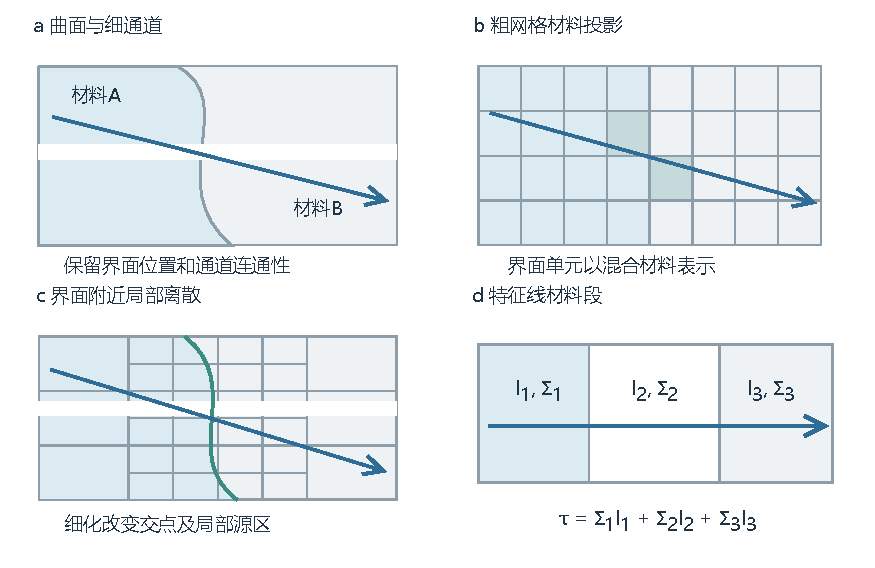
\includegraphics[width=0.95\linewidth]{figures/fig1}
\caption{非贴体材料表示与特征线分段\upcite{7--10}}
\label{fig:1}
\end{figure}

\begin{figure}[htbp]
\centering
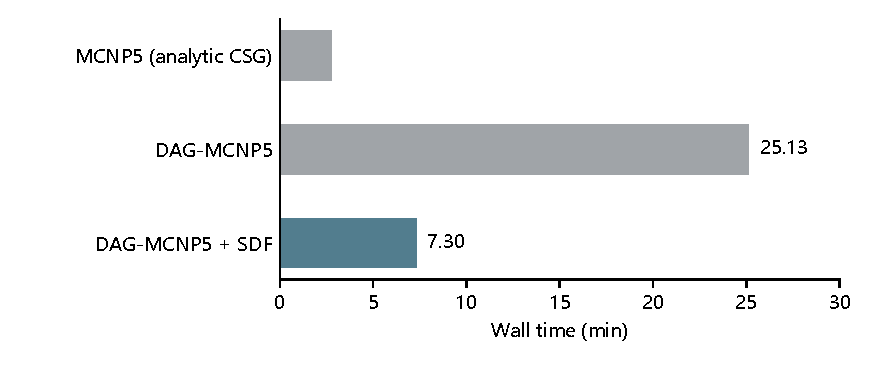
\includegraphics[width=0.95\linewidth]{figures/geometry_sdf}
\caption{SDF辅助几何追踪的计算时间比较\upcite{64}}
\label{fig:sdf}
\end{figure}

规则体素通过整数索引访问材料与源区数据，局部细化则提高指定区域的空间分辨率。块结构方法将细化单元放在矩形块内，用连续数组保存各块的数据，再由层级索引处理粗细网格的关系。AMReX中的Box、BoxArray和DistributionMapping分别描述矩形区域、块集合及其并行分配，重网格时依据标记聚类形成新块，再迁移数据\upcite{11}。GPU自适应笛卡尔网格研究还分析了相邻网格层级差异的控制、网格并行构建及动态更新所需的计算开销\upcite{12}。对中子输运，块的计算负载还与穿越特征线数量、段长分布、能群和迭代次数相联系，因此工作量估计可以超出单元数量本身。

\subsection{体素穿越与几何界面求交方法}

均匀体素的材料定位可由坐标、网格原点和步长计算整数索引。Amanatides与Woo的快速遍历算法维护射线到下一组$x,y,z$网格面的参数值及各轴的增量，每次选择最小参数并更新相应索引\upcite{68}。原文给出相邻体素推进所需的两次浮点比较与一次加法。这一计数针对基本推进操作，不包含初始化、材料读取和输运计算。在MOC中，该算法根据射线起点、方向和网格尺寸，依次确定射线经过的体素，并计算每个体素内的射线段长度。面、棱、角交点的相等参数需一致处理，防止零长度段、漏段或重复段。相邻同材料体素可共享衰减计算，但应保留源区和通量统计区的分界。采用CMFD加速时，还需单独记录粗网界面的中子流。

局部细化改变单元尺寸，均匀DDA的固定轴向增量因而不能直接贯穿所有层级。Laine与Karras用稀疏八叉树保存表面附近的体素，在每个节点记录八个子节点是否存在，并利用相对地址定位子节点，减少树结构的存储量\upcite{69}。用于中子输运时，可沿八叉树逐层定位射线穿过的叶单元，即不再细分的空间单元，并读取该单元的尺寸和材料编号。中子输运需要继续追踪穿过真空孔道和多层材料的射线，并为相应源区计算通量。八叉树用于输运时，需保留这些区间及源区信息，同时记录树节点存储、地址访问和跨层定位的计算成本。

层次包围盒（BVH）将CAD面元按空间位置分组，用逐层嵌套的包围盒建立树结构。射线追踪时，先检查射线是否与包围盒相交，排除不相交盒内的面元，再对剩余候选面元求交。随后对交点排序并判断所处实体，得到材料边界与材料编号。体素与几何界面结合的追踪方法可在界面单元中使用BVH辅助求交，在其余单元中采用规则体素穿越。后续实验将分别测量材料段长度误差、候选面元数量和求交时间，评价界面精度与几何追踪开销的关系。图\ref{fig:2}比较三种操作，区分材料定位、叶单元穿越和表面求交的输入输出。

\begin{figure}[htbp]
\centering
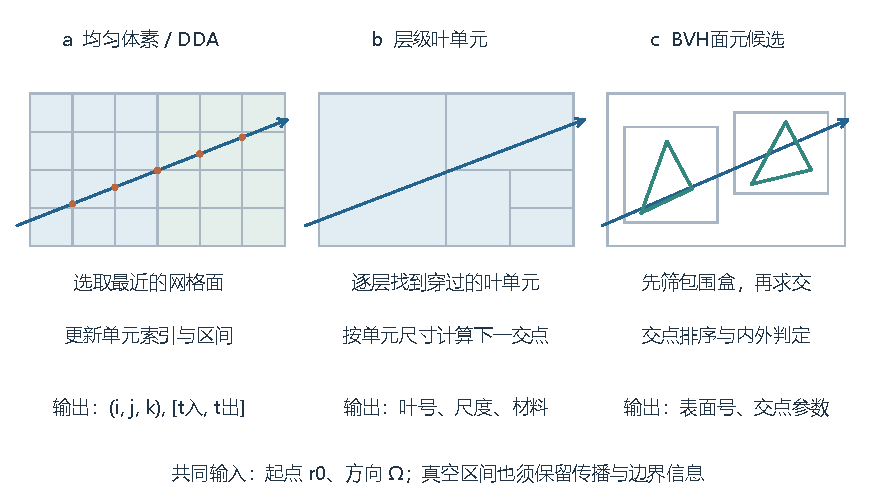
\includegraphics[width=0.95\linewidth]{figures/dda_index}
\caption{DDA、八叉树与BVH射线追踪示意}
\label{fig:2}
\end{figure}

\subsection{MOC空间离散与目标导向自适应}

MOC把指定方向的输运方程转化为沿射线的一维递推。射线与材料界面及源区边界的交点将其划分为多个段。每段需要总截面、长度和源项的近似表示。对给定能群、离散方向和源迭代步，以下将总角源\(Q_g[\psi]+q_g\)简记为\(Q\)，它是每单位立体角的源，已包含散射与外源的角向归一化。各向同性标量源\(S_g\)对应\(Q=S_g/(4\pi)\)。各向异性散射以所采用阶次的角矩重建并记录其截断阶。段内截面和\(Q\)均为常数时，出射角通量由

\begin{equation}
\psi_{out} = \psi_{in}e^{- \Sigma_{t}l} + \frac{Q}{\Sigma_{t}}(1 - e^{- \Sigma_{t}l})
\label{eq:3}
\end{equation}

给出，其中\(l\)为材料段长，\(\Sigma_{t} > 0\)。真空极限\(\Sigma_{t} \rightarrow 0\)取\(\psi_{out} = \psi_{in} + Ql\)。小光学厚度下采用稳定的指数差计算。段平均角通量及其对源区标量通量的贡献可写为
\begin{equation}
\begin{aligned}
\bar\psi_{kns}&=\frac{Q}{\Sigma_t}+\left(\psi_{\rm in}-\frac{Q}{\Sigma_t}\right)\frac{1-e^{-\tau}}{\tau},\quad \tau=\Sigma_t\ell_{kns},\\
\phi_r&\simeq\frac{1}{V_r}\sum_n w_n\sum_{(k,s)\in r}a_{kn}\ell_{kns}\bar\psi_{kns}.
\end{aligned}
\label{eq:tally}
\end{equation}
式中各量均对应同一能群，\(n,k,s\)分别表示离散方向、轨迹和轨迹子段，\(w_n\)为角权重（和为\(4\pi\)），\(a_{kn}\)为与角权重分开的射线横截面求积权重，\(V_r\)为源区体积。每个方向的轨迹横截面权重与段长之积用于近似源区体积，并按源区体积归一化得到标量通量。反应率由相应空间区内的标量通量与宏观反应截面相乘后积分得到。真空段平均值取\(\psi_{\rm in}+Q\ell/2\)，小光学厚度采用指数差或级数保持稳定。特征线需要在材料、源项近似或通量统计区域发生变化的位置分段。相邻区间即使具有相同材料和源值，也应分别计算各源区的通量积分。采用粗网有限差分（CMFD）加速时，还需记录穿过粗网界面的中子流。扫描中可共享相同区间的衰减计算，但应保留各空间区的通量积分和界面中子流，再据此更新散射源及加速方程。由此，几何交点决定材料段，源区划分决定沿程源近似，轨迹间距和角向求积决定积分分辨率。

OpenMOC包含二维CSG射线追踪、平源MOC、源迭代和粗网有限差分加速，并以C5G7和LRA问题检验本征值与功率分布\upcite{13}。Gaston等在MOCkingbird中采用非结构网格三维长特征线，使完整轨迹穿过多个计算子域，并比较预先保存分段与求解时重新分段两种方法。其全堆芯算例达到约14亿单元、12000个处理器\upcite{14}。局部细化增加射线与网格的交点，产生更多需要保存和扫描的短段。轨迹跨越计算子域时，还要传递边界角通量。因此，评价三维MOC的存储与运行时间时，需要同时统计网格单元数、轨迹段数和跨域传输量。

Porhemmat等在二维MOC中采用模块化射线追踪（Modular Ray Tracing，MRT），利用重复栅元的局部追踪结果，减少同类几何的重复求交和轨迹存储\upcite{66}。该研究比较了三种角向求积。在Legendre--Chebyshev $S_{20}$设置下，C5G7正向和伴随计算与参考$k_{\mathrm{eff}}$之差分别为$7\times10^{-6}$和$9\times10^{-6}$，16个CPU线程的加速比为6.18。聚变孔道和曲面部件的几何重复程度与规则栅元不同，后续研究将统计可复用的模块数量，并测量读取已有轨迹与重新生成轨迹分别需要的时间。

Liu等在多层八叉树上建立非匹配笛卡尔网格，用于离散纵标计算，随后发展了随通量解变化的预测--校正方法，利用通量形状和平衡关系计算粗细网格界面上的通量\upcite{10,15}。这些研究表明，局部加密既要生成不同尺寸的网格，也要计算粗细网格间传递的通量，并安排满足依赖关系的扫描顺序。MOC沿轨迹把上一段的出射角通量传给下一段，可据此检查粗细单元交界处是否存在漏段、重复段或通量不连续。

自适应的另一核心问题是依据什么量分配分辨率。标准误差指标强调全域解或局部梯度。目标导向方法使用伴随信息，把残差对探测器或积分响应的贡献作为加密依据。Wang与Ragusa在二维非结构三角形网格上比较高阶DG的标准与目标导向自适应，讨论点通量和区域平均反应率。Lathouwers针对体与表面探测器构造含角度依赖的双重加权残差及目标误差控制\upcite{16,17}。远端探测区的绝对通量可能很小，目标导向选择使误差控制与需要评价的响应直接对应。

Baker等在球谐角展开和空间子网格尺度有限元框架中，用子网格校正构造残差，并组合正向、伴随各向异性误差度量，针对两个单群和一个多群固定源屏蔽问题选择加密位置\upcite{18}。Goffin等把目标泛函扩展到有效增殖因子\upcite{19}。这些研究将“哪里需要分辨率”具体化为与空间格式、残差构造和目标定义相联系的数值过程。对MOC开展类似研究时，可从源区重构误差、段积分及轨迹积分残差入手，构造与其离散一致的目标指标。

Liu等的后续工作分别推进了全局与目标精度控制。2022年研究利用多层金字塔结构、空间矩比指标和扫描优化，在达到相同精度时，相对均匀细化节省60\%---80\%的计算成本。2023年研究以加权差分通量重构残差，并以DWR驱动多群固定源与临界问题的加密，在所测目标相近精度下减少超过70\%的工作量和运行时间\upcite{20,21}。在Balakovo-3固定源剂量基准中，多层八叉树将约950万网格降至190万，对传统离散纵标计算和实验结果的RMS差异分别约为4\%与10\%，相对均匀细网格节省约70\%计算成本\upcite{22}。这些结果为采用局部细化减少达到指定响应精度所需的工作量提供了依据。

近年的发展还包括提高空间阶次。Wilson等将非连续等几何离散、目标误差度量、局部\(h(p)\)细化与扩散加速结合，在参考空间求解后投影形成误差估计\upcite{23}。这使网格划分具有改变单元尺寸和提高解表示阶次两种选择。表\ref{tab:1}按数值处理与验证结果归纳代表性工作。后续研究可以比较细化、源展开和界面重构各自减少的误差及其计算代价。 \begin{longtable}{@{}>{\raggedright\arraybackslash}p{\dimexpr0.24\linewidth-1.5\tabcolsep\relax}>{\raggedright\arraybackslash}p{\dimexpr0.22\linewidth-1.5\tabcolsep\relax}>{\raggedright\arraybackslash}p{\dimexpr0.24\linewidth-1.5\tabcolsep\relax}>{\raggedright\arraybackslash}p{\dimexpr0.28\linewidth-1.5\tabcolsep\relax}@{}}
\caption{复杂几何与目标导向空间离散的代表性研究}\label{tab:1}\\
\toprule
工作 & 对象与离散 & 数值处理 & 验证结果及启发 \\
\midrule
\endfirsthead
\toprule
工作 & 对象与离散 & 数值处理 & 验证结果及启发 \\
\midrule
\endhead
\bottomrule
\endlastfoot
Amanatides--Woo，Laine--Karras\upcite{68,69} & 规则体素DDA，稀疏表面八叉树 & 增量式跨网格面，掩码与相对寻址 & 前者生成体素区间，后者借鉴层级定位，均需补充体材料与源区信息 \\
Shriwise\upcite{64} & 氢球点源蒙卡，$10^8$历史 & SDF预筛选下一边界查询 & 原DAGMC墙钟25.13 min降至7.30 min，解析CSG为2.75 min \\
Gaston\upcite{14} & 非结构网格三维MOC全堆芯 & 完整轨迹与跨域角通量传递 & 约14亿单元、12000处理器，分别统计网格单元数和轨迹存储量 \\
Porhemmat\upcite{66} & C5G7二维MOC & 模块化追踪与求积比较 & 16 CPU线程加速6.18倍，复用条件取决于几何重复性 \\
Chen，Yang\upcite{7,8} & CAD-MOC，CAD至离散纵标网格 & 通用射线求交，体积加权混合材料 & 几何边界访问与材料投影分别进入输运离散 \\
Buchan\upcite{9} & 内部实体与独立背景有限元网格 & supermeshing守恒投影并结合自适应 & 分别控制实体边界和背景求解网格的分辨率 \\
Baker，Lathouwers\upcite{17,18} & 固定源探测器，有限元或DG & 正伴随误差度量，含角度依赖的DWR & 按目标积分控制加密位置及停止条件 \\
Liu 2020/2021\upcite{10,15} & 八叉树非匹配笛卡尔$S_N$ & 层级扫描、预测—校正通量映射 & 局部细化同时需要粗细界面传递 \\
Liu 2022\upcite{20} & 多层空间矩离散 & 空间矩比指标与优化扫描 & 相同精度下较均匀细化节省60\%--80\%成本 \\
Liu 2023 DWR\upcite{21} & 三维多群固定源与临界 & 加权差分重构残差及近似伴随 & 相近目标精度下工作量和时间减少$>$70\% \\
Liu 2023 Balakovo\upcite{22} & VVER-1000固定源剂量 & 多层网格、源投影与跨界映射 & 约950万$\rightarrow$190万网格，对计算/实验RMS约4\%/10\% \\
Wilson 2026\upcite{23} & 非连续等几何$S_N$ & 目标度量、$h(p)$细化与扩散加速 & 在光滑制造解中检查空间阶次，并按目标误差选择细化位置 \\
\end{longtable}

DWR为双重加权残差，RMS为均方根差异。

\subsection{已有研究的联系与待解决问题}

CAD材料映射确定每个空间单元的材料，射线追踪计算特征线经过哪些单元及各段长度，MOC再利用段长、截面和源项递推角通量。孔道在材料映射中被错误封闭，会改变整条射线经过的材料。局部网格细化则增加交点和扫描段数。因此，后续研究将分别测量材料路径误差、空间源近似误差和实际扫描段数，比较提高响应精度所需的时间与显存。

\section{GPU-MOC与高性能并行计算研究现状}\label{sec:3}

\subsection{MOC并行计算与轨迹的生成和存储}

GPU-MOC将大量轨迹---能群任务分配给并行线程，在给定源项下完成沿程扫描，再汇集各空间单元的通量贡献。单条轨迹中，后一段的入射角通量来自前一段出射值，计算具有沿程次序。不同轨迹、离散方向和能群可分别分配给并行线程。每个线程承担的计算量由轨迹段数、能群数和边界通量传递共同决定。同一线程束内的轨迹段数差异较大时，短轨迹对应线程会等待其余线程完成。按段数或估计计算量对轨迹分组，可以减少线程等待。

轨迹信息可全部预先保存、在扫描时生成，或只保存其中一部分。预先保存的方法把段长、材料编号和源区编号存入数组，每次源迭代直接读取。在线生成的方法在扫描时重新追踪射线，减少段数组的存储量，但增加求交计算。部分缓存则保留重复使用较多或生成较慢的轨迹，其余轨迹按需生成。Song等在少群三维MOC中结合线性源、在线轴向追踪和分批扫描，使计算能够在单GPU上运行\upcite{24}。Zhou等比较缓存部分轨迹与在线生成其余轨迹的方法\upcite{25}。比较三种存储方法时，应记录每次扫描的生成时间、读取时间和同时占用的显存，并观察源迭代次数变化后的总时间。

通用射线追踪逐段计算几何交点，适用于CAD或体素几何\upcite{7}。MRT则利用重复几何，保存模块内的局部轨迹及连接关系，扫描时重复使用这些局部数据\upcite{66}。显式存储能复用首次追踪的结果，在线生成需要在每次扫描时执行追踪。两者的时间差由交点数量、每次追踪的计算量、显存读取速度和复用次数共同决定。

多条特征线可以并行扫描，但它们经过同一源区时，需要把各自的通量积分加到同一个结果中。直接使用原子加法可以保证并行更新正确，当大量线程同时写入同一地址时，部分更新会等待。线程块内先求和、再写入全局通量数组，可以减少全局原子加次数，同时需要共享内存和线程同步。NVIDIA的线程束聚合示例及CUDA指南分别介绍了聚合原子更新、合并访存和数据复用的方法\upcite{26,27}。本研究将统计同一源区的写入次数，比较直接原子加与局部求和的时间。图\ref{fig:3}显示轨迹扫描、缓存读取、通量求和与源更新的先后关系。

\begin{figure}[htbp]
\centering
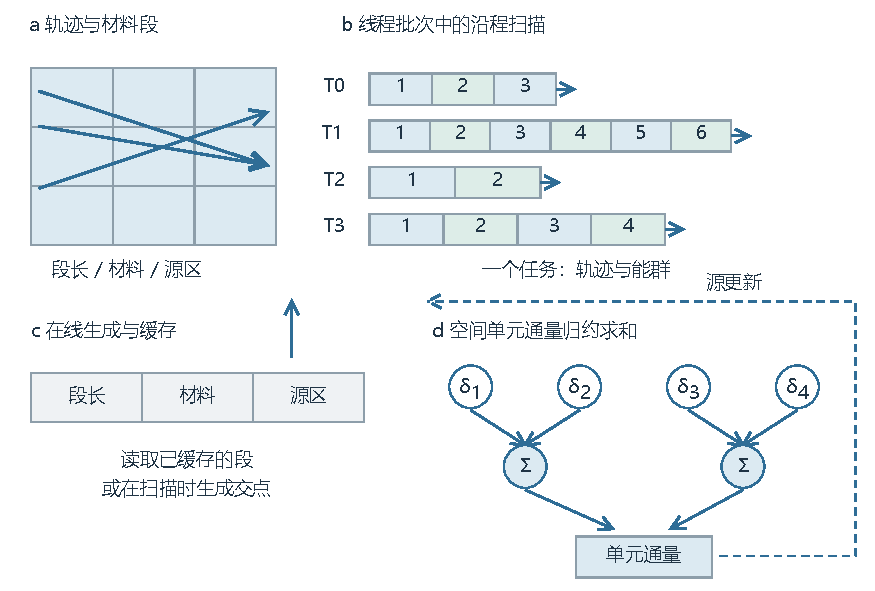
\includegraphics[width=0.95\linewidth]{figures/fig3}
\caption{GPU-MOC轨迹扫描与通量求和\upcite{24--26,28--31}}
\label{fig:3}
\end{figure}

OpenMOC在二维C5G7七群问题中，把能群计算放在内层以使用向量指令，并将轨迹--能群任务分配给CUDA线程。研究比较4至128个方位角，在四种NVIDIA GPU上的最大求解加速比接近单Xeon核的50倍。随着方位角增加，可并行的任务数量增加，GPU相对于CPU的加速比也随之提高\upcite{13}。宋佩涛等采用通信与GPU扫描重叠、异步数据传输和CPU/GPU任务分配，减少异构MOC计算中的等待时间\upcite{28,32}。

Wang等针对轴向挤出几何采用循环轨迹分解，把轨迹划分为比单纯角度分解更小的任务，再按估计计算量分配给处理器。在ORISE上从10240扩展到98304个CPU核时，并行效率保持在40\%以上\upcite{33}。汪岸进一步研究周期几何中的轨迹长度分布及任务分配\upcite{34}。ANT-MOC将存储、计算和通信开销用于节点、GPU及计算单元三个层次的负载分配，在16000个DCU上报告70.69\%的强扩展效率和89.38\%的弱扩展效率，处理的轨迹数量约为$10^{11}$\upcite{29}。对一般体素材料场，可以逐条统计段数和材料访问量，检验这些量能否预测各设备的运行时间。

\subsection{GPU计算性能与正向--伴随求解}

三维求解中的显存占用包括轨迹段、源项、标量与角通量、散射矩、边界数据及迭代工作区。对轴向挤出问题，在线轴向追踪利用径向轨迹与轴向平面的交点生成三维段。分批扫描则控制同时驻留的轨迹数据。Song等的OpenMOC扩展先以平源、显式三维段存储建立基线：仅25 cm高组件即需22129 MB显存。线性源通过提高空间近似阶次减少所需分段。在线轴向追踪保留二维段、在扫描时生成三维交点。分批处理进一步限制轨迹及边界通量的同时驻留量。组合后组件显存较原配置降低98.5\%，并以蒙卡生成的四群截面完成单GPU的SMR全堆芯计算\upcite{24}。线性源、在线追踪和分批处理分别减少空间自由度、轨迹段存储和同时驻留的边界通量。比较这些方法时，需要分别测量各项改动及其组合对显存和运行时间的影响。对于体素几何，在线DDA也可消除显式段数组，但其几何定位代价与该文利用轴向挤出结构的追踪不同。

Dzianisau与Lee在STREAM3D-GPU中结合MOC/DD、轴向分解和异步执行，将每个MPI进程的GPU存储由理论约50 GB降至4.5 GB以下，8和16个GPU的MOC/DD求解分别较128核CPU参考快22.1和40.5倍\upcite{30}。其2024年KNS报告说明轴向分解的具体操作：扫描前从主机传入当前平面所需入射通量，扫描后回传出射通量和CMFD网格界面中子流，保留可复用的设备数据。该研究表1的七群、64轴向平面C5G7，在两颗EPYC 7543的64核参考与同主机加8块RTX A5000之间，MOC时间由1368 s降为34 s，总时间由1704 s降为100 s。该研究表2的72群、197平面OPR-1000八分之一堆芯，MOC时间由61535 s降为3995 s，总时间由212416 s降为11201 s\upcite{35}。前一算例的总时间缩短倍数小于扫描时间缩短倍数，后一算例的总时间还受MPI径向分区等待时间变化的影响。轴向分解通过控制驻留数据缓解容量限制，异步执行能否使传输与计算重叠则仍取决于传输量与计算量。这两份研究分别采用八分之一堆芯和四分之一堆芯。

NuDEAL在轴向挤出几何上采用MOC/HFEM和DGMOC，在一般多面体网格上采用DFEM-$S_N$，通过减少需保存的角通量和逐批扫描方位角控制显存占用\upcite{31}。其三维C5G7算例含8507520个单元，采用RTX 2080 Ti。每个角度块从2角增加到32角时，显存由2589 MB增加到7133 MB，单次输运扫描由5.25 s缩短到5.09 s，单次MOC步骤由10.50 s缩短到9.21 s。64角同时扫描时显存不足。图\ref{fig:4}根据公开作者稿arXiv:2607.01591v1表6绘制，比较每块2、4、8、16和32角的结果。增加同批计算的角度会增大工作数组，在该算例中显存增加约1.75倍，而扫描时间仅缩短约3\%。因此，选择每批角度数时，需要同时测量显存占用和扫描时间。其二维DFEM-$S_N$算例在同一RTX 4070 Ti上，并发计算与顺序计算的总时间分别为26 s和148 s。

STRAUM将多群离散纵标计算移到GPU上，采用群块Krylov迭代和空间波前扫描，计算Kobayashi问题与压力容器屏蔽问题\upcite{36}。Gong等研究了GPU上的三维离散纵标输运计算\upcite{37}。这些固定源问题可用于比较不同扫描顺序、能群迭代和并行任务划分对运行时间的影响。

GPU输运还覆盖时间依赖与大型工程求解。Zou等在ALPHA中实现全隐式瞬态固定源MOC，采用棒级CMFD，以C5G7-TD和MPACT作结果对照，并研究FP32及MOC收敛容限\upcite{38}。Denovo则以GMRES和空间---角度---能量并行求解大型固定源问题，在Titan的K20x节点上用于JET中子学\upcite{39}。这两类研究分别提供源随时间更新和大规模外源传播的实现参照。表\ref{tab:2}将计算对象、并行计算方法及对应结果放在同一比较框架中。

OpenSn提供多群离散纵标输运的开源求解程序\upcite{40}。其源迭代、空间扫描和并行求解实现可作为程序开发的参照。Pryer将波前扫描用于批量输运计算，研究同一设备上同时处理多个样本的方法\upcite{41}。混合计算中也可以分别选择运行确定论和蒙卡的设备，Biondo等介绍的Shift流程在CPU上完成Denovo正向及伴随计算、权窗生成和源偏倚，在GPU上进行蒙卡输运及权窗控制\upcite{42}。

\Needspace{0.70\textheight}
\begin{longtable}{@{}>{\raggedright\arraybackslash}p{\dimexpr0.21\linewidth-1.5\tabcolsep\relax}>{\raggedright\arraybackslash}p{\dimexpr0.16\linewidth-1.5\tabcolsep\relax}>{\raggedright\arraybackslash}p{\dimexpr0.27\linewidth-1.5\tabcolsep\relax}>{\raggedright\arraybackslash}p{\dimexpr0.34\linewidth-1.5\tabcolsep\relax}@{}}
\caption{并行MOC及GPU固定源输运的算法与计算结果}\label{tab:2}\\
\toprule
工作 & 计算对象 & 并行计算方法 & 主要结果与计算条件 \\
\midrule
\endfirsthead
\toprule
工作 & 计算对象 & 并行计算方法 & 主要结果与计算条件 \\
\midrule
\endhead
\bottomrule
\endlastfoot
OpenMOC\upcite{13} & 二维组件输运 & 轨迹/能群并行与CUDA扫描 & 四种NVIDIA GPU测试，相对单Xeon核最大求解加速近50倍 \\
宋佩涛等\upcite{28} & 二维异构并行MOC & 通信与GPU扫描重叠 & 异步传输并分配CPU/GPU工作量，减少通信等待 \\
ANT-MOC\upcite{29} & 直接三维堆芯输运 & 三级任务分配及存储/通信模型 & 16000个DCU：强/弱扩展效率70.69\%/89.38\% \\
Wang等\upcite{33} & 挤出几何三维CPU并行 & 循环轨迹与组合负载分配 & 10240$\rightarrow$98304 CPU核，并行效率$>$40\% \\
Song等\upcite{24} & 少群三维组件/SMR & 线性源、在线轴向追踪、分批 & 组件显存降低98.5\%，支持单GPU四群全堆芯 \\
STREAM3D-GPU\upcite{30} & OPR-1000三维MOC/DD & 轴向分解与异步执行 & 8/16 GPU对128核CPU求解22.1/40.5倍，每进程$<$4.5 GB \\
NuDEAL\upcite{31} & DGMOC及DFEM-$S_N$ & 角通量压缩与角度分块 & 3D C5G7，RTX 2080 Ti：每块2/32角：2589/7133 MB，单扫5.25/5.09 s \\
STRAUM\upcite{36} & 压力容器固定源 & 群块Krylov与空间波前 & 比较能群划分和扫描方法对GPU运行时间的影响 \\
\end{longtable}

图\ref{fig:4}显示同一算例中改变角度块大小的影响，表\ref{tab:2}分别列出其他研究的计算对象与方法。GPU-MOC运行时间主要包括轨迹生成与读取、沿程扫描、通量求和、源更新和设备间传输。后续实验将分项测量这些时间，并统计每项同时占用的显存。

\begin{figure}[htbp]
\centering
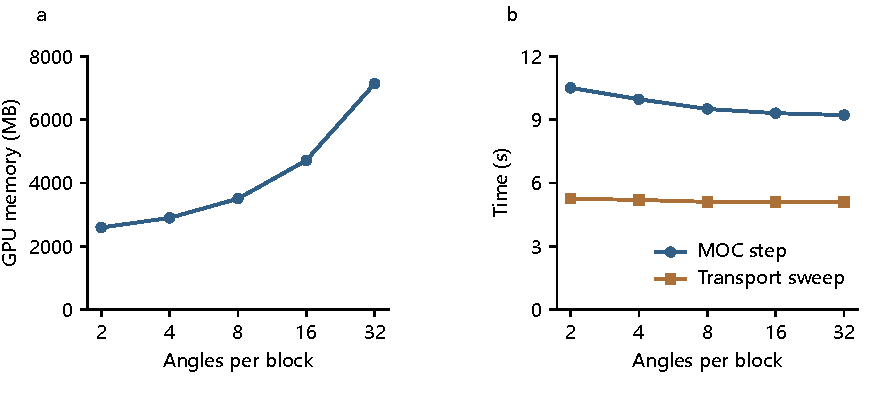
\includegraphics[width=0.95\linewidth]{figures/fig4_nudeal}
\caption{NuDEAL角度块大小对显存和计算时间的影响\upcite{31}}
\label{fig:4}
\end{figure}

伴随输运将目标响应作为源，其计算需要转置散射和能群耦合关系，并按照配对边界条件反向扫描特征线。对实数离散矩阵\(A\)及由正体积、正求积权等构成的对称正定内积矩阵\(W\)，离散伴随满足

\begin{equation}
A^{\dagger} = W^{- 1}A^{\mathsf{T}}W,\langle Au,v\rangle_{W} = \langle u,A^{\dagger}v\rangle_{W}.
\label{eq:4}
\end{equation}

实现时可共享材料、轨迹及源区索引，将正向散射源更新替换为对应转置运算，并使轨迹传播和边界数据交换服从伴随次序。可用内积对偶关系和源---响应互易关系检查离散实现，再将得到的重要性场用于第五章的权窗计算\upcite{5,43}。正向与伴随求解将分别通过内积关系检验，再比较GPU加速后的运行时间。

\subsection{复杂体素几何中的计算与存储问题}

现有GPU-MOC研究通过压缩轨迹、在线生成和分批扫描减少显存占用，并把轨迹、方向和能群分配给不同线程。聚变模型中的薄层、斜界面和孔道会使不同轨迹穿过的单元数差异很大。局部细化增加几何查询次数，而相邻同材料区间是否需要分段还取决于源区和通量统计区域。因此，分配线程任务时，需要根据实际扫描段数和访存量估计计算量，并检查长轨迹造成的等待。

本研究将在相同材料、射线和收敛要求下，比较显式存储、在线生成和部分缓存的运行时间。外源值变化时，几何交点通常可以继续使用。材料或几何改变时，则需检查材料编号、段长和源区编号是否仍有效。第四章将据此设计轨迹缓存、线程分组和通量求和的对照实验。

\section{体素化MOC与GPU协同加速的研究思路}\label{sec:4}

体素尺寸改变源区数量和射线段数，GPU扫描则反复读取这些段的长度、材料编号和源值。网格细化对响应精度的改善，因而会伴随存储量和扫描时间的变化。本研究分别研究体素材料路径误差、GPU扫描方法，以及网格细化与GPU参数的联合选择，再用聚变屏蔽及成熟减方差方法检验应用效果。

\subsection{RQ1：复杂几何体素化及特征线输运}

\textbf{研究依据与问题。}Chen等的CAD-MOC、Buchan等的非贴体材料投影和Liu等的层级空间离散分别处理了几何求交、材料表示与局部计算资源分配\upcite{7,9,10,15,20--22}。这些研究提示，需要区分几何近似误差与在给定几何上求解输运方程的离散误差。拟研究的问题是：在薄层、斜界面和孔道附近，体素材料标记改变了哪些路径的光学厚度，这些变化如何传递到指定响应。局部细化在等显存或等墙钟时间条件下是否仍优于均匀细化？

\textbf{路径误差与初步假设。}以可解析的CAD/CSG材料模型为参照，对同一射线起点和方向分别求精确材料区间与体素区间。将二者交点取并集，可在共同参数区间上比较材料及截面。对轨迹\(k\)、能群\(g\)，定义
\begin{equation}
\tau_{kg}=\sum_j\Sigma_{t,g,m_j}\ell_j,\qquad
\Delta\tau_{kg}=\tau^{h}_{kg}-\tau^{\mathrm{ref}}_{kg},\qquad
E_{\tau,kg}=\sum_{J}\left|\Sigma^{h}_{t,g,J}-\Sigma^{\mathrm{ref}}_{t,g,J}\right|\ell_J.
\label{eq:patherror}
\end{equation}
这里\(h\)表示体素网格的划分，\(J\)为共同分段。\(E_{\tau}\)避免不同材料误差相互抵消。同一正入射角通量下，纯吸收无源段有\(\psi_{\rm out}=\psi_{\rm in}e^{-\tau}\)，因此\(\psi^h_{\rm out}/\psi^{\rm ref}_{\rm out}=e^{-\Delta\tau}\)。存在散射和体源时，响应还取决于源项分布及方向积分，因此还要测量源区和角向离散误差。

本研究拟优先细化对目标响应影响较大的薄层和孔道，与均匀细化比较相同预算下的响应误差。细化位置同时考虑材料界面和响应灵敏度。窄孔道若被体素材料标记封闭，将改变传播路径，因此实验将检查孔道连通性，并测量逐材料段长、光学厚度误差及响应变化。

\textbf{方法、对照与控制变量。}从均匀体素和DDA穿越建立基线，再比较局部块细化和层级体素。采用解析CSG或可直接访问CAD表面的几何追踪方法建立材料段参考，比较纯体素追踪与界面单元求交的段长误差及运行时间。材料映射以中心点标记为基础对照，按需要增加子采样体积分数。混合材料必须明确截面均匀化和源区处理约定。依次改变体素尺度、界面相对网格的平移、倾角、薄层厚度与孔道宽度。固定物理材料、射线集合、核数据、边界和迭代容限。先在无散射解析问题中测路径误差，再在同一映射几何上收敛轨迹间距、角度、源展开和迭代，以隔离不同误差来源。

分别按距材料界面的距离、通量变化和目标加权残差选择细化位置，并比较三种方法。目标导向指标借鉴已有\(S_N\)方法\upcite{16--18,21}，但需对MOC离散建立残差和伴随配对。初期可通过局部扰动计算响应灵敏度，比较不同位置细化后的误差变化。评价采用相对响应误差、边界中子流与守恒残差、路径误差分位数、体素/源区数量、构建时间和显存。在相同显存或计算时间预算下，比较各局部细化方法的目标响应误差。联合改变空间与角向分辨率，识别角向误差占主导时继续细化空间网格的效果。

\subsection{RQ2：GPU-MOC并行算法及性能优化}

\textbf{研究依据与问题。}OpenMOC、Song等、ANT-MOC、STREAM3D-GPU与NuDEAL分别展示了能群并行、轨迹压缩或重建、任务分配、轴向分解和角度分批的不同作用\upcite{13,24,28--31,35}。拟研究在复杂体素几何中，轨迹长度与段数分布如何改变缓存对运行时间的影响及线程负载，并确定不同源迭代次数下，在线生成与轨迹缓存各自适用的显存和时间范围。

\textbf{需要保存和统计的量。}对第\(k\)条射线，分别记录访问体素数\(N_{v,k}\)、材料段数\(N_{m,k}\)、源积分子段数\(N_{q,k}\)、计分子段数\(N_{t,k}\)和实际扫描段数\(N_{s,k}\)。材料、源项近似或通量统计区域改变时，应保留相应分段。相邻体素即使材料相同，各源区的通量积分仍要分别计算。只有合并前后各空间区的积分相同，才能共用沿程衰减计算。细化网格后，增加的体素访问、源积分和通量求和可能具有不同数量，因此将分别统计这些操作的计算量。

段长、材料编号、源区编号和轨迹起始位置分别保存在连续数组中，并与把这些量放在同一结构体中的方法比较。对同一组射线，分别保存全部轨迹、全部在线生成或缓存部分轨迹，测量生成与读取的时间。缓存内容按方向或空间块划分，另外比较按复用次数选择缓存轨迹的方法。外源值、材料编号和源区划分分别改变时，检查哪些段长及索引仍可复用，哪些需要重新生成。

\textbf{线程分配与通量求和实验。}同一线程束内的任务段数越接近，短任务等待长任务的时间可能越少。实验将比较原始轨迹顺序、按段数分组和按空间位置分组，同时测量排序时间与访存速度。对通量求和，比较直接原子加、线程块内先求和及分阶段求和，记录全局原子加次数、共享内存和同步时间。每条轨迹仍按入射到出射的顺序递推角通量，跨线程或跨设备划分轨迹时，明确传递上一段出射通量的时间与方式。

固定射线、群结构、源迭代容限和浮点精度，先单独改变缓存，再改变分组与求和，随后检验交互作用。CPU串行、多线程及GPU版本使用同一离散模型。误差比较覆盖响应、通量范数、守恒与对累积顺序的敏感性。计时拆为轨迹生成、主机--设备传输、扫描、通量求和、源更新和同步。GPU异步内核采用设备事件及同步后的端到端墙钟时间。指标包括有效内存带宽、线程束内负载差异、高频原子写入位置、峰值显存、每秒扫描的段数与达到收敛要求的总时间。性能分析器计数与无分析器的重复计时分开，避免采样开销污染结果。

\subsection{RQ3：体素化与GPU执行协同优化}

\textbf{研究问题与假设。}局部细化可减少达到指定精度所需的源区数量，同时改变不同轨迹的段数分布。减小每个角度批次的大小能够降低驻留显存，但会增加批次数量及调度开销。本研究拟分析空间细化、轨迹缓存和任务分组之间的相互影响，比较独立选择与联合选择这些参数时的完整求解时间。图\ref{fig:cost}给出网格、轨迹段数与计算成本之间的关系。

\begin{figure}[htbp]
\centering
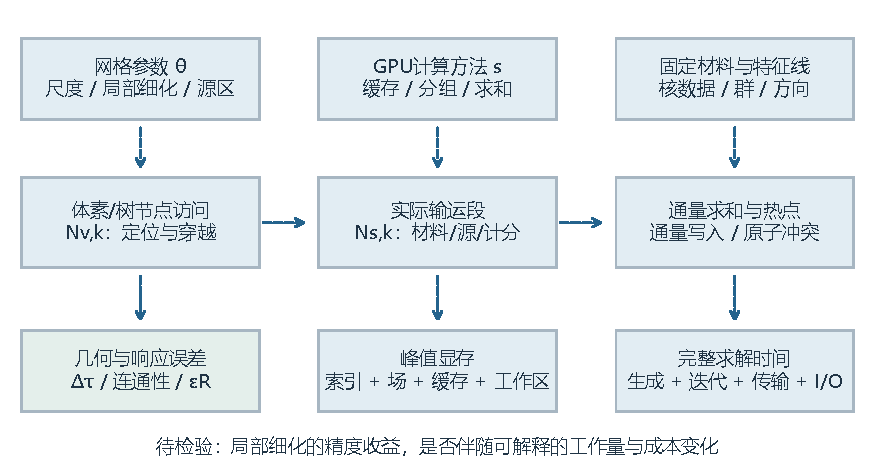
\includegraphics[width=0.95\linewidth]{figures/voxel_gpu_cost}
\caption{体素离散与GPU计算成本的关系}
\label{fig:cost}
\end{figure}

\textbf{运行时间与显存模型。}以\(\theta\)表示体素尺寸、细化位置和源区划分，以\(s\)表示轨迹缓存比例、线程分组和通量求和方法。在固定能群和射线集合下，分别记录准备、迭代和输出时间，并记录计算过程中同时驻留显存的数据量：
\begin{equation}
\begin{aligned}
T(\theta,s)&=T_{\rm setup}+\sum_{i=1}^{N_{\rm it}}T_{{\rm iter},i}+T_{\rm IO},\\
T_{{\rm iter},i}&=T_{{\rm track},i}+T_{{\rm transfer},i}+T_{{\rm sweep},i}
 +T_{{\rm reduce},i}+T_{{\rm source},i},\\
M_{\rm peak}&=\max_{t\in\mathcal T}\sum_{a\in\mathcal A(t)}M_a.
\end{aligned}
\label{eq:cost}
\end{equation}
\(T_{\rm setup}\)包含材料映射、初始追踪及初始传输。每次迭代的\(T_{{\rm track},i}\)和\(T_{{\rm transfer},i}\)累计该步所有批次实际发生的在线生成、缓存重建与传输。在线追踪嵌入扫描内核时，单独测量或估计其耗时，避免重复计时。各阶段时间之和对应计算与通信没有重叠的实现。采用异步执行时，以设备事件和同步边界测得的关键路径时间评价完整成本。\(\mathcal A(t)\)为时刻\(t\)仍驻留显存的数据与缓冲区集合，包括体素/索引、源/通量、驻留轨迹、工作区和双缓冲，工作区复用只计实际分配一次。扫描预测从\(G\sum_kN_{s,k}\)出发，另引入每个线程束的最大工作量、实际访问字节数和热点区域的求和次数。在线生成成本与\(\sum_kN_{v,k}\)及层级节点访问数关联。\(G\)为能群数，\(N_{\rm it}\)采用各配置实际达到收敛要求的迭代次数。

在给定响应误差容限和显存预算下，选择网格与GPU参数的问题可写为
\begin{equation}
\min_{\theta,s}\ T(\theta,s),\qquad
\max_{d\in\mathcal D}\frac{|R_d(\theta,s)-R_d^{\rm ref}|}{a_d+|R_d^{\rm ref}|}\leq\varepsilon_R,
\qquad M_{\rm peak}(\theta,s)\leq M_{\rm budget}.
\label{eq:joint}
\end{equation}
\(\mathcal D\)为计算前选定的响应集合，\(a_d\)为近零响应采用的有量纲绝对尺度。对每组网格和GPU参数，先检查响应误差与显存是否满足要求，再比较完整求解时间。

\textbf{联合选择网格与GPU参数。}以均匀体素和显式轨迹存储为基准，比较只改变网格、只改变GPU方法、两者分别选择后组合及同时选择四组结果。实验变量包括体素尺寸、细化位置、缓存比例、线程分组和求和方法。先在小模型上逐组测量，得到满足精度和显存要求的最短求解时间，再检验成本模型能否选出接近这一结果的参数组合。

用部分几何及参数组合拟合成本模型，再用未参与拟合的孔道、倾角和细化位置检验预测结果。评价时间预测误差、所选参数相对实测最优参数多耗费的时间，以及不满足精度或显存要求的比例。更换GPU时重新测量带宽和调度开销。通过这些比较，确定哪些轨迹特征可以解释运行时间，以及模型适用于哪些几何和设备。

\subsection{实验矩阵与实施次序}

\begin{longtable}{@{}>{\raggedright\arraybackslash}p{\dimexpr0.12\linewidth-1.5\tabcolsep\relax}>{\raggedright\arraybackslash}p{\dimexpr0.27\linewidth-1.5\tabcolsep\relax}>{\raggedright\arraybackslash}p{\dimexpr0.27\linewidth-1.5\tabcolsep\relax}>{\raggedright\arraybackslash}p{\dimexpr0.28\linewidth-1.5\tabcolsep\relax}@{}}
\caption{核心研究问题与验证方法}\label{tab:rq}\\
\toprule
问题 & 变量与对照 & 固定条件与观测量 & 支持或否定假设的判据 \\
\midrule
\endfirsthead
\toprule
问题 & 变量与对照 & 固定条件与观测量 & 支持或否定假设的判据 \\
\midrule
\endhead
\bottomrule
\endlastfoot
RQ1 & 均匀/块细化/层级，中心标记/子采样，界面位置与角度 & 同射线及核数据，逐材料段长、$E_\tau$、连通性、响应误差 & 同显存或同时间下误差降低，检查角向误差是否限制空间细化的效果 \\
RQ2 & 显式/在线/部分缓存，原顺序/按段数分组，原子加/局部求和 & 同离散与精度，段数分位数、线程等待时间、带宽、显存、全迭代时间 & 节省的时间超过排序/重建/同步耗时，通量与守恒满足CPU/GPU一致性 \\
RQ3 & 只改网格、只改GPU方法、分别选择后组合、联合选择 & 同响应集合及预算，实测最快参数、预测误差、所选参数多耗费的时间 & 在未参与拟合的几何上满足精度要求并缩短总时间，分析预测失效的原因 \\
应用 & 固定成熟CADIS/FW-CADIS，改变MOC网格与求解参数 & 同MC几何和核数据，均值、RSD、权窗与达到目标精度的总时间 & 保持统计一致性，完整成本改善可归因于快速场求解 \\
\end{longtable}

\begin{figure}[htbp]
\centering
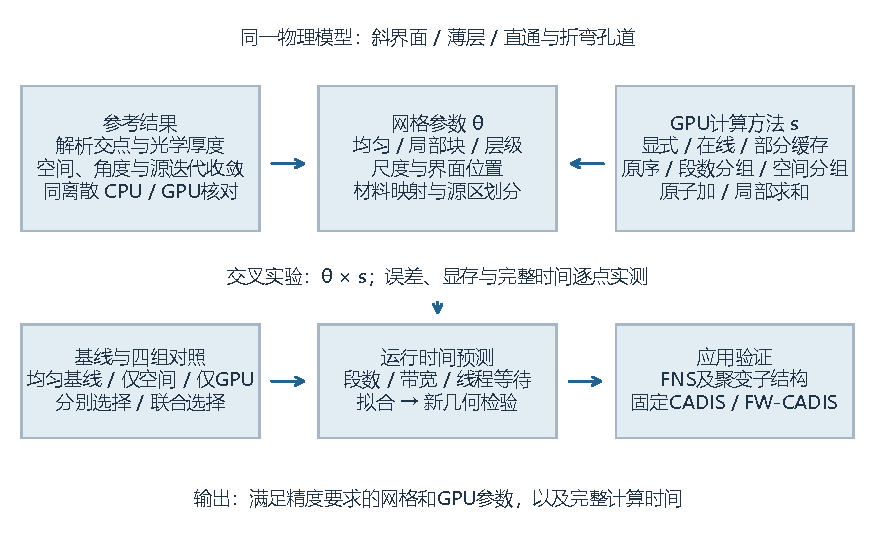
\includegraphics[width=0.95\linewidth]{figures/research_design}
\caption{研究技术路线与实验设计}
\label{fig:design}
\end{figure}

\section{聚变屏蔽算例验证与减方差应用}\label{sec:5}

\subsection{体素化MOC与GPU计算的分层验证}

本研究以中子固定源通量、泄漏率和反应率为主要验证量。FNS基准中的产氚率用作特定中子反应率的实验检验，相关加热响应按基准定义分别评价。光子加热和瞬发光子剂量作为中子--光子耦合扩展，停堆剂量及活化--衰变链作为成熟耦合方法的文献背景。表\ref{tab:5}列出文献中的中子响应及光子加热响应（GHR）。本研究先验证中子响应，开展中子--光子耦合计算时再评价GHR。

验证依次回答材料段是否正确、离散解是否收敛、GPU执行是否与CPU一致，以及工程响应是否可信。第一层使用均匀纯吸收体、多材料平板及可解析斜界面，检查射线进出点、段长总和、材料次序和指数衰减。对薄层和孔道移动网格原点，检验细小结构被体素漏标或错误连通的条件。局部细化还需核对粗细界面的唯一定位，避免重复或遗漏射线区间。

第二层固定体素材料模型，独立收敛轨迹间距、角度求积、空间源展开和源迭代。再用几何更精确或更细的参考模型测体素近似误差。参考程序比较采用相同核数据和能群约定。连续能蒙卡可补充物理参考，但其统计误差和多群凝聚差异应单列，不能全部归为MOC空间误差。

第三层在完全相同的离散输入上核对CPU/GPU通量、响应、边界中子流与守恒残差，检查不同轨迹顺序和求和方法的浮点敏感性。单GPU先比较全流程时间与峰值显存。多GPU扩展再固定全局问题规模或每设备工作量，分别报告强/弱扩展、通信与最慢任务时间。设备型号、软件版本、精度、收敛阈值和全部计时边界随结果保存。第四、五层分别进入实验基准和聚变子结构，之后才评价快速场解的减方差应用。

\subsection{屏蔽基准与聚变工程研究}

实验基准提供了从物理模型到可测响应的检验。SINBAD由NEA与RSICC共同维护，覆盖反应堆、聚变和加速器屏蔽。其材料与孔道实验为屏蔽程序提供实验对照\upcite{59}。对于本研究，FNS材料实验和孔道实验分别提供高能中子在实体材料中衰减与在低密度通道中传播的对象，可以将空间与角度近似放到不同物理条件下考察。

Ebiwonjumi等采用OpenMC 0.14.1-dev分析FNS钨、钒和铍组件，使用约14 MeV D-T源，以能谱、反应率、光子加热和产氚率与实验及MCNP 6.2比较\upcite{1}。钨例采用Denovo/MAVRIC生成的权窗，钒和铍例按较小组件直接开展计算。输运核数据使用ENDF/B-VII.1，相应剂量学反应使用IRDFF截面。光子谱按探测器能量分辨展宽后比较。表\ref{tab:5}列出其产氚和加热响应的整体C/E结果，其中C/E指计算值除以实验值，所附离散度为不同测点C/E的标准差。作者稿表VIII--IX给出的未舍入均值与标准差分别为1.0295与0.1956（铍TPR，9点）、0.9537与0.1366（钨和钒GHR，共7点）。这些是未按实验不确定度加权的测点汇总，不能代替各深度处的C/E比较。

车锐等采用cosRMC计算FNS-Duct和FNS-W基准，并与MCNP5及实验中子谱比较\upcite{60}。FNS-Duct的折弯通道用于检验孔道传播及壁面散射，FNS-W用于检验钨屏蔽中的能谱变化。Iwamoto等采用PHITS和JENDL-4.0计算FNS铁屏蔽，在0.003--10 MeV积分中子产额上，六个位置的C/E为1.15--1.78\upcite{61}。

Ibrahim等将CAD蒙卡与CADIS/FW-CADIS用于ITER中子学计算，评价线圈核热、屏蔽外剂量和通量分布\upcite{62}。其后续网格研究在两次均为10天、权窗文件约0.21 GB的MCNP计算中，将非零计分比例由79.3\%提高到97.8\%，对应非零计分元素数相对增加23.3\%\upcite{51}。确定论空间--能量单元由1640万增加到5.28亿，权窗经粗化保留1630万空间--能量单元。以全局网格平均相对方差定义的MC FOM提高3.4倍。确定论求解网格细化可改善重要性场，而权窗粗化减少蒙卡查询所需的存储，因此两个阶段可以采用不同网格。

Lu等在CFETR线圈屏蔽分析中采用密度降低减方差方法，先在较低密度模型上形成权窗，再逐步恢复实际密度，最终在物理密度下计算线圈核响应\upcite{2}。Zhang等在cosRMC中研究多层网格自适应全局减方差\upcite{55}。这类研究可作为材料更新和多层权窗应用的比较对象。

Royston等采用Denovo开展大型聚变中子学固定源计算，研究空间、角度和能群并行在工程模型中的应用\upcite{39}。

Moreno等用ParaStell生成WISTELL-D的99组包层与高温屏蔽模型，并用OpenMC比较氚增殖和磁体核热。在2113 MW聚变源功率下，研究中的厚型、增殖层占比60\%的设计点得到TBR为1.10、磁体总核热为152.0 kW\upcite{3}。Liew与Ku将三维蒙卡、二维离散纵标和一维近似结合，用于CIT试验大厅的材料和厚度选择\upcite{63}。
\begin{longtable}{@{}>{\raggedright\arraybackslash}p{\dimexpr0.19\linewidth-1.5\tabcolsep\relax}>{\raggedright\arraybackslash}p{\dimexpr0.37\linewidth-1.5\tabcolsep\relax}>{\raggedright\arraybackslash}p{\dimexpr0.22\linewidth-1.5\tabcolsep\relax}>{\raggedright\arraybackslash}p{\dimexpr0.20\linewidth-1.5\tabcolsep\relax}@{}}
\caption{聚变屏蔽基准与工程研究的对象和结果}\label{tab:5}\\
\toprule
研究对象 & 计算方法与条件 & 评价响应 & 代表性结果 \\
\midrule
\endfirsthead
\toprule
研究对象 & 计算方法与条件 & 评价响应 & 代表性结果 \\
\midrule
\endhead
\bottomrule
\endlastfoot
FNS钨/钒/铍\upcite{1} & OpenMC、ENDF/B-VII.1，约14 MeV源，钨例用Denovo权窗 & 能谱、反应率、GHR、TPR & 9个TPR测点平均C/E=\allowbreak1.03$\pm$0.20，7个GHR测点0.95$\pm$0.14 \\
FNS-Duct /\newline FNS-W\upcite{60} & cosRMC中子--光子输运，MCNP5及实验对照 & 中子通量谱 & 比较孔道传播、壁面散射与钨中能谱变化 \\
FNS铁体\upcite{61} & PHITS/JENDL-4.0，FNS铁屏蔽实验 & 0.003--10 MeV积分中子产额 & 六位置C/E为1.15--1.78，表列不确定度为计数统计 \\
ITER多响应\upcite{62} & CAD蒙卡与CADIS/FW-CADIS & TFC核热、屏蔽外剂量、通量 & 采用局部及全局重要性服务不同响应 \\
ITER自适应剂量图\upcite{51} & 同为10天MCNP、约0.21 GB权窗 & 设施网格非零计分覆盖 & 79.3\%$\rightarrow$97.8\%，非零计分元素数量相对增23.3\% \\
CFETR线圈\upcite{2} & 密度降低与迭代权窗，最终恢复物理密度 & 线圈核热与快中子注量 & 比较不同屏蔽材料和厚度的线圈核响应 \\
CFETR全局权窗\upcite{55} & cosRMC多层网格减方差 & 网格通量统计 & 研究多层权窗对全局计分的影响 \\
WISTELL-D设计扫描\upcite{3} & ParaStell/DAGMC/OpenMC，99组，2113 MW源 & TBR与磁体总核热 & 厚型/60\%增殖层设计点：1.10、152.0 kW \\
CIT试验大厅\upcite{63} & 三维MC与二维$S_N$辅助一维计算 & 屏蔽材料及厚度 & 用多维输运结果校正近似模型 \\
\end{longtable}

GHR为光子加热响应，TPR为产氚率。FNS平均C/E的±为测点间标准差，非单次蒙卡计分误差。TFC为环向场线圈。

\subsection{工程响应、误差来源与方案更新}

表\ref{tab:5}中的工程与实验研究涉及不同计分对象，实际应用需要预先明确响应的位置、物理权重和归一化。磁体总核热是整个区域的能量沉积积分，局部热功率密度则需要保留空间峰值。快中子注量和绝缘剂量对应不同能量权重。维护区的瞬发剂量与冷却后的停堆剂量还涉及不同源项。FNS实验中的每源粒子结果可与测量归一化比较，工程功率和注量再按物理源强及运行时间换算。因此，全局通量图、指定探测器和磁体局部计分应分别设置精度目标，并在同一模型中检查。

误差评价将物理偏差与抽样不确定度分开报告。FNS研究中，钒的低能中子谱、钨的部分阈反应和近源加热存在不同程度的C/E偏差，其变化与核数据、探测器、源表示和测量条件有关\upcite{1}。对数值方法的比较可以固定这些输入，观察空间与角度离散参数引起的响应变化。与实验比较时，则保留材料成分、源谱、探测器响应和实验不确定度。这样的安排可以把算法改进对应到具体误差来源。

对图\ref{fig:7}各层次对象的方案更新，需要依据数据的物理依赖关系处理。几何不变时，改变外源主要影响正向场及源偏倚。在固定输运算子和单一目标下，伴随解可继续表示该目标的重要性。FW-CADIS的加权伴随源还依赖正向响应。改变材料会改变截面与输运算子，移动孔道则同时改变交点和传播路径。拟分别记录源、材料和几何三类更新的数据重建范围，以实际完成各方案响应所需的时间评价数据复用效率。

\subsection{聚变屏蔽实验与子结构验证}

拟按图\ref{fig:7}所示的对象层次建立算例。先以解析材料段和可计算交点的几何核对特征线及材料映射，再采用均匀体、多层材料和直通或折弯孔道，分别改变层厚、界面倾角、孔道宽度和弯折位置。各算例固定物理源与响应，先完成所采用空间、角度和能量离散参数的收敛比较，再将直接蒙卡、MAGIC及适合该目标的混合方法放在一致输入下评价。

\begin{figure}[htbp]
\centering
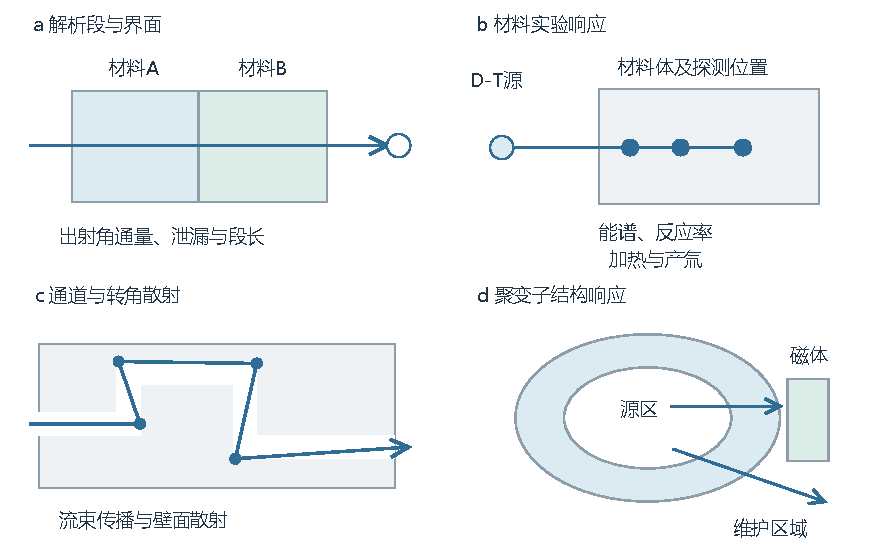
\includegraphics[width=0.95\linewidth]{figures/fig7}
\caption{材料段、屏蔽基准与聚变子结构验证\upcite{1,2,59,60,62}}
\label{fig:7}
\end{figure}

随后选取可获取输入的FNS材料与通道基准，保存条目版本、材料密度和成分、源谱与角分布、核数据库、反应截面及探测器定义。能谱比较使用相同能区划分和相应探测器分辨，反应率与核热按一致的每源粒子及质量或体积归一化。对每个响应给出C/E、实验不确定度和蒙卡统计误差，并以独立程序结果作交叉比较。数值收敛、程序交叉与实验符合度各提供一层证据。

工程应用拟以磁体屏蔽或维护孔道子结构为对象，比较源、材料/层厚和孔道更新。各方法统一响应精度、计分规则与资源预算，记录首次准备、重建及达标时间，形成可复现算例。

算例统一核数据约定：输运多群截面拟由FENDL-3.x或ENDF/B-VIII.0连续能量库按选定能群结构凝聚，能群结构在开题阶段结合基准算例与响应类型确定。剂量学与活化反应采用IRDFF等配套评价截面。



\subsection{伴随驱动的源偏倚与权窗}

减方差的目标是用有限粒子历史获得所需响应的统计精度。源偏倚改变粒子出生状态的抽样概率。分裂增加对目标有贡献的粒子分支数量。俄罗斯轮盘减少低贡献粒子的后续计算。每项操作均通过权重修正，使保留历史在期望上代表原来的物理源。权窗以空间和能量区间规定粒子的适宜权重范围，为输运中的分裂和轮盘提供依据。

伴随输运为这种资源分配提供目标相关信息。令\(L\)为线性固定源输运算子，\(q\)为物理源，\(d\)为目标响应函数。在配对边界条件下，正向与伴随问题满足

\begin{equation}
L\psi = q,L^{\dagger}\psi^{\dagger} = d,R = \langle d,\psi\rangle = \langle q,\psi^{\dagger}\rangle.
\label{eq:5}
\end{equation}

这里的内积包含空间、能量和角度积分。伴随角通量\(\psi^{\dagger}\)描述某一位置、能量和方向上的粒子对指定响应的期望贡献。Wagner与Haghighat利用离散纵标伴随解，为蒙卡构造一致的源偏倚和权窗，形成CADIS方法\upcite{4}。Munk与Slaybaugh的综述将此类确定论驱动方法与蒙卡迭代、角度相关方法纳入共同的技术谱系\upcite{44}。

为区分物理源强与抽样概率，设\(\int_{}^{}{p(x)dx} = 1\)，\(x\)表示被偏倚的源变量，\(I(x)\)为源支持集上的正重要性近似。定义

\begin{equation}
C = \int_{}^{}{p(x)I(x)dx},\widehat{p}(x) = \frac{p(x)I(x)}{C},w_{0}(x) = \frac{p(x)}{\widehat{p}(x)} = \frac{C}{I(x)}.
\label{eq:6}
\end{equation}

按\(\widehat{p}\)抽样后，以\(w_{0}\)修正出生粒子的权重，计算结果再按物理源强归一化。重要性较高的源状态被更频繁地抽样，同时赋予较小权重。输运权窗的目标权重也由同一\(I\)的倒数确定，使出生权重与沿程权重控制相互一致。上下限和存活权重由具体程序的窗宽约定设置。MAVRIC中的Denovo---Monaco流程实现了这一关系\upcite{43}。ORNL的ADVANTG把Denovo伴随解到CADIS/FW-CADIS参数的生成自动化，与MAVRIC同属生产级工具链，是本计划耦合流程的直接参照\upcite{67}。

对多个探测器或大范围计分，FW-CADIS利用一次正向计算估计各目标的响应，并以这些估计调节伴随源\upcite{5}。对于预先给定的响应函数\(d_{i}\)、正的估计\({\widetilde{R}}_{i}\)及无量纲优先级\(\beta_{i}\)，可以对归一化目标\(\sum_{i}^{}{\beta_{i}R_{i}/{\widetilde{R}}_{i}}\)构造

\begin{equation}
d_{FW} = \sum_{i = 1}^{N_{D}}\frac{\beta_{i}}{{\widetilde{R}}_{i}}d_{i}.
\label{eq:7}
\end{equation}

预计响应较低的目标因而获得较高的伴随源权重。不同目标仍按各自响应定义计分。用于全局通量、区域剂量或探测器能谱的伴随源，应与对应的空间和能量权重一致。图\ref{fig:5}比较单目标CADIS和正向加权FW-CADIS的计算次序，以及二者共同的源偏倚与权窗关系。

\begin{figure}[htbp]
\centering
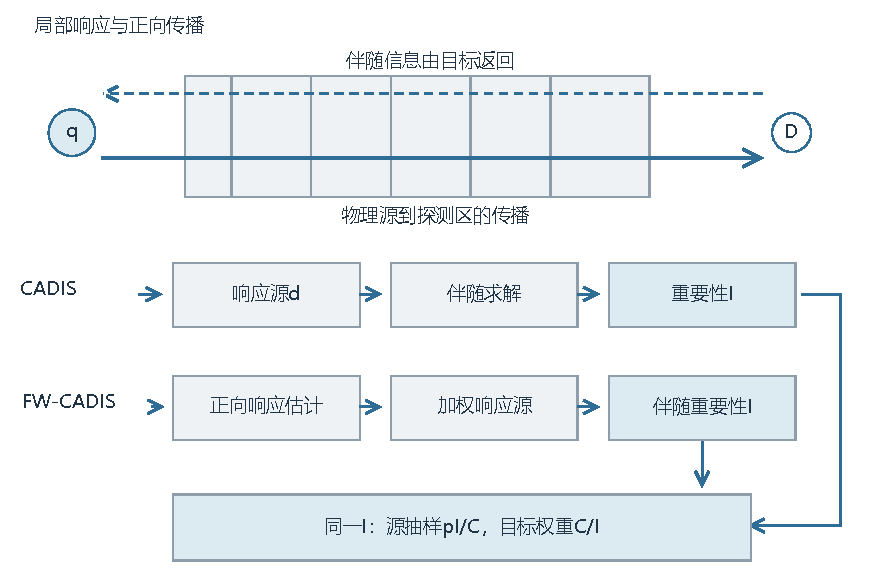
\includegraphics[width=0.95\linewidth]{figures/fig5}
\caption{CADIS与FW-CADIS重要性生成及源偏倚\upcite{4,5,43}}
\label{fig:5}
\end{figure}

角度相关方法进一步处理同一空间---能量状态中方向不同的贡献。Munk等在CADIS-Ω中以正向角通量加权伴随角通量，构造

\begin{equation}
I_{\Omega}(r,E) = \frac{\int_{4\pi}^{}{\psi(r,E,\Omega)\psi^{\dagger}(r,E,\Omega)d\Omega}}{\int_{4\pi}^{}{\psi(r,E,\Omega)d\Omega}}.
\label{eq:8}
\end{equation}

该量是在有正向通量的状态上定义的角度加权标量重要性，能够把前向流束与目标贡献的方向关系引入空间---能量权窗\upcite{45}。

Munk等在混凝土迷宫中比较CADIS与CADIS-$\Omega$。标量伴随场主要描述位置和能量的重要性，正向角通量则给出实际粒子传播的方向分布。CADIS-$\Omega$用后者加权伴随角通量，使权窗随孔道中的主要传播方向变化\upcite{45}。这种计算需要同时保存或积分正向与伴随角通量，可用于检查忽略方向信息对孔道重要性估计的影响。

Zhao等的LAA-CADIS采用局部角度适应，面向复杂通道改进重要性计算\upcite{46}。这两类研究使角向信息的作用可以通过流道中的传播方向、探测器能区和权窗执行分别考察。

多步骤响应则需要在不同物理阶段之间传递重要性。MS-CADIS针对停堆剂量，沿中子照射、活化和衰变光子输运的联系，将最终剂量的重要性传回中子抽样阶段\upcite{47}。其关键是按最终响应分配前一步的统计投入。对瞬发核热、运行剂量和冷却后的停堆剂量，需要分别选取相应的响应链和核数据。

\subsection{重要性生成、权窗优化与计算效率}

自动权窗既可由近似输运解生成，也可由蒙卡逐次探索形成。Davis与Turner将MAGIC用于ITER全局分布计算，通过已有蒙卡通量与统计信息迭代更新重要性和权窗\upcite{48}。随机射线方法则在多群、固定源区表示下随机选取起点和方向，沿射线积分并迭代通量。正向及伴随场可以用于CADIS/FW-CADIS。OpenMC现行流程同时提供MAGIC和内置随机射线权窗生成，支持在同一几何中完成权窗预计算和蒙卡生产输运\upcite{49}。表\ref{tab:3}比较这些方法所需信息与对应响应。 \par
\Needspace{0.70\textheight}
\begin{longtable}{@{}>{\raggedright\arraybackslash}p{\dimexpr0.22\linewidth-1.5\tabcolsep\relax}>{\raggedright\arraybackslash}p{\dimexpr0.22\linewidth-1.5\tabcolsep\relax}>{\raggedright\arraybackslash}p{\dimexpr0.21\linewidth-1.5\tabcolsep\relax}>{\raggedright\arraybackslash}p{\dimexpr0.33\linewidth-1.5\tabcolsep\relax}@{}}
\caption{自动减方差方法的信息来源与响应构造}\label{tab:3}\\
\toprule
方法 & 重要性信息来源 & 对应响应 & 主要计算步骤 \\
\midrule
\endfirsthead
\toprule
方法 & 重要性信息来源 & 对应响应 & 主要计算步骤 \\
\midrule
\endhead
\bottomrule
\endlastfoot
CADIS\upcite{4} & 目标响应的伴随场 & 单个或明确局部响应 & 响应源$\rightarrow$伴随$\rightarrow$一致源偏倚与权窗 \\
FW-CADIS\upcite{5} & 正向响应加权的伴随场 & 多探测器、区域或全域 & 正向估计$\rightarrow$加权响应源$\rightarrow$伴随$\rightarrow$权窗 \\
CADIS-$\Omega$\upcite{45} & 正向角通量加权伴随 & 局部方向性贡献 & 正/伴随角信息$\rightarrow$替代标量重要性 \\
LAA-CADIS\upcite{46} & 局部角度自适应 & 复杂通道响应 & 按局部方向贡献改善重要性 \\
MS-CADIS\upcite{47} & 跨物理步骤的伴随联系 & 指定冷却时刻停堆剂量 & 衰变光子目标$\rightarrow$活化$\rightarrow$中子重要性 \\
MAGIC\upcite{48,49} & 前次蒙卡通量及统计信息 & 全局粒子分布 & 探索输运$\rightarrow$更新权窗$\rightarrow$继续迭代 \\
随机射线CADIS/FW-CADIS\upcite{49,50} & 多群随机射线正向/伴随场 & 局部或全局响应 & 源区与MGXS准备$\rightarrow$射线迭代$\rightarrow$一致偏倚 \\
\end{longtable}

MGXS为多群截面。随机射线是场求解方式，可用于构造CADIS或FW-CADIS重要性。

计算重要性场和蒙卡查询权窗对网格的要求不同。Ibrahim等分别采用材料宏观化、确定论网格细化和权窗粗化，在重要区域提高场解分辨率，并控制权窗文件大小\upcite{51}。郑华庆等将自动网格和权窗平滑用于屏蔽计算\upcite{52}。NECP-MCX利用NECP-Hydra正向与伴随计算生成权窗，并研究按贡献粗化权窗网格\upcite{53,54}。Zhang等在cosRMC中采用多层网格生成全局权窗\upcite{55}。

材料均匀化改变通道中的有效截面，角向求积决定主要传播方向的分辨率，权窗映射决定粒子跨越网格时采用的目标权重。THETA使用线性源随机射线方法，在单元内表示源项的空间变化\upcite{56}。后续应用实验将分别改变源区尺寸和源展开阶次，比较重要性场精度、内存和预计算时间。

Raffuzzi等在SCONE中采用随机射线生成CADIS/FW-CADIS权窗，并以混凝土屏蔽及源--探测器问题与MAGIC和直接蒙卡比较\upcite{50}。其整体屏蔽的P0平源计算中，20次独立运行得到仅计蒙卡时间的FOM为1.08$\pm$0.14 min$^{-1}$，加入权窗生成时间后为0.96$\pm$0.12 min$^{-1}$。两种计时结果的差别直接反映预计算对总成本的影响。表\ref{tab:4}列出这些研究的算例、计时条件与数值结果。
\begin{longtable}{@{}>{\raggedright\arraybackslash}p{\dimexpr0.24\linewidth-1.5\tabcolsep\relax}>{\raggedright\arraybackslash}p{\dimexpr0.21\linewidth-1.5\tabcolsep\relax}>{\raggedright\arraybackslash}p{\dimexpr0.37\linewidth-1.5\tabcolsep\relax}>{\raggedright\arraybackslash}p{\dimexpr0.16\linewidth-1.5\tabcolsep\relax}@{}}
\caption{重要性计算与权窗输运的代表性结果}\label{tab:4}\\
\toprule
研究及算例 & 比较内容 & 文献报告值 & 对应的计算环节 \\
\midrule
\endfirsthead
\toprule
研究及算例 & 比较内容 & 文献报告值 & 对应的计算环节 \\
\midrule
\endhead
\bottomrule
\endlastfoot
ITER网格与权窗\upcite{51} & 同为10天MCNP，权窗文件约0.21 GB & 非零计分79.3\%提高到97.8\%，MC FOM提高3.4倍 & 材料宏观化、求解网格细化与权窗粗化 \\
Raffuzzi整体屏蔽\upcite{50} & RR-FW-CADIS的P0平源，20次独立运行 & 仅MC FOM为1.08$\pm$0.14，含WW生成为0.96$\pm$0.12 min$^{-1}$ & 权窗生成与生产输运的分别计时 \\
Shift先进架构\upcite{58} & CPU历史型与GPU事件型权窗输运 & Frontier两例在20节点上MC运行$<$2 min，每GCD吞吐为最佳CPU实现9--11倍 & GPU计算芯片GCD的粒子执行与队列调度 \\
\end{longtable}

Raffuzzi等结果的$\pm$为20次完整运行之间的标准差，WW为权窗。各行采用对应研究的FOM和计时定义。

粒子执行成本还取决于权窗引起的分裂规模。一条较大权重历史进入较低目标权重区域时，可以产生大量后代。其他并行任务完成后，尚未结束的长历史可能延长墙钟时间。Turner与Davis据此提出动态调整该历史权窗的长历史处理，并以包括并行效率的指标评价参数\upcite{57}。Evans等则在Shift中比较CPU历史型线程和GPU事件型执行，使权窗控制与不同硬件上的粒子队列相适应\upcite{58}。这里需要同时观察方差、每条源历史的工作量与其他任务等待长历史结束的时间。

对单个响应，常用蒙卡效率和完整计算时间可分别表示为

\begin{equation}
{FOM}_{MC} = \frac{1}{{RSD}^{2}T_{MC}},T_{all} = T_{prep} + T_{\det} + T_{WW} + T_{MC} + T_{IO}.
\label{eq:9}
\end{equation}

其中，\(T_{prep}\)包含实际发生的几何和核数据准备，\(T_{\det}\)包含所需正向与伴随求解，\(T_{WW}\)为映射、生成与处理权窗的时间，\(T_{IO}\)为输出和数据管理时间。各项按实际边界计时，避免重复累计。全局评价还需指定计分集合、相对方差的汇总方式和零计分处理。生产输运中的原始源历史是统计单位，其分裂后代的贡献在同一历史中汇总。这样可以把重要性生成、权窗执行和最终响应可靠性放在同一评价中。

\subsection{混合减方差应用的受控比较}

在体素化MOC和GPU固定源求解经过验证后，拟用成熟CADIS/FW-CADIS与MAGIC流程评价快速场解的应用效果。重点比较不同MOC网格和GPU参数生成的重要性是否保留主要贡献通道，以及预计算时间的降低能否转化为达到目标精度的总计算时间的改善。先固定物理几何、材料、源和响应集合，在材料多群截面及其生成约定一致的条件下，分别改变源区细度、角向求积和源展开。每次记录重要性沿主要通道的分布、权窗存储、粒子权重与源历史工作量，再比较局部响应的RSD和达到目标精度的总计算时间。图\ref{fig:6}给出分层试验路线。

\begin{figure}[htbp]
\centering
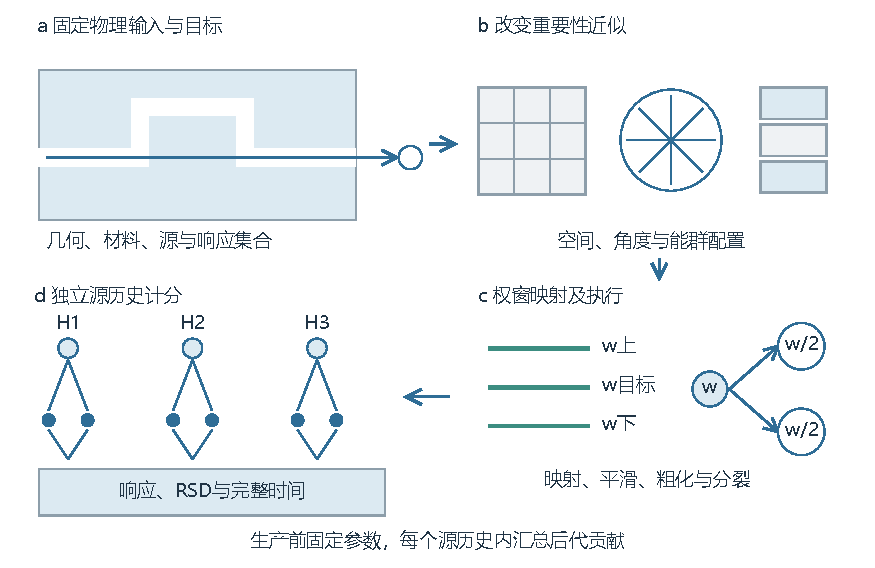
\includegraphics[width=0.95\linewidth]{figures/fig6}
\caption{确定论--蒙卡耦合减方差验证\upcite{49--51,54,57,58}}
\label{fig:6}
\end{figure}

固定预计算场后，仅以预先选定的成熟映射、粗化和平滑规则开展敏感性对照，分离场近似与权窗表示各自产生的效率变化。LAA-CADIS、贡献粗化和MAGIC作为外部方法参照。应用计算采用固定的权窗规则，重点评价MOC场解精度和预计算时间对蒙卡统计效率的影响。

场到权窗接口确定坐标单位、MOC源区与能群边界、MC权窗网格及能量分段。采用固定的空间分片常数查询和按既定群边界重分组。跨越多个MC材料区的权窗单元只提供抽样重要性，生产碰撞与几何仍使用原MC模型。对同一场单独改变映射规则时，分别报告响应均值、RSD、每源历史工作量、文件大小与达标时间。源支持必须完整覆盖。未覆盖区域先补齐映射，非物理负值先核对离散求解或投影，未通过检查的场不用于源偏倚。对零值及舍入级小负值，使用与重要性同单位、按参考正值尺度预先规定的下限\(\epsilon_I>0\)，令\(I_\epsilon=\max(I,\epsilon_I)\)，重新计算\(C_\epsilon=\int pI_\epsilon dx\)、\(\widehat p_\epsilon=pI_\epsilon/C_\epsilon\)及\(w_{0,\epsilon}=C_\epsilon/I_\epsilon\)。权窗上下限与存活权重均按同一处理后重要性和固定窗宽约定设置。分裂权重总和、轮盘期望权重及抽样概率归一化逐项核对。关键响应与直接MC或独立成熟权窗在预设置信区间内比较均值一致性，再评价RSD与时间。

正式比较前固定权窗及参数，将生成、调参与生产计分分开记录。达标时间采用预先指定的误差与稳定性规则，并以独立完整重复计算核查均值和方差。再通过源更新、材料更新及孔道移动组成的序列，考察哪些重要性或轨迹数据可以复用、何时需要重新计算。应用结论限定为快速MOC场解在所选屏蔽任务中的适用性，以及预计算节省在完整成本中的占比。权窗映射与平滑采用固定的成熟规则。若预计算已非主要成本，应据实报告GPU场求解对总时间的贡献范围。


\section{博士阶段拟开展的研究工作}\label{sec:6}

\subsection{程序开发与阶段安排}

研究首先开展体素化MOC程序开发，建立包含几何输入、材料映射、特征线追踪、源区积分和多群源迭代的CPU参考实现，并完成边界条件、收敛性和守恒检验。在此基础上开发GPU固定源扫描算法，研究轨迹存储、任务分配与通量求和。应用阶段先采用成熟工具提供伴随参考解，再通过离散算子及配对边界检验，将伴随求解迁移至MOC程序。

按四年博士培养周期提出表\ref{tab:6}的工作安排，具体时间结合源码条件和培养要求调整。各阶段按解析验证、数值收敛、GPU性能和工程算例的顺序开展，以前一阶段的结果作为后续研究的基础。

\begin{longtable}{@{}>{\raggedright\arraybackslash}p{\dimexpr0.14\linewidth-1.5\tabcolsep\relax}>{\raggedright\arraybackslash}p{\dimexpr0.29\linewidth-1.5\tabcolsep\relax}>{\raggedright\arraybackslash}p{\dimexpr0.29\linewidth-1.5\tabcolsep\relax}>{\raggedright\arraybackslash}p{\dimexpr0.22\linewidth-1.5\tabcolsep\relax}@{}}
\caption{博士阶段研究内容与预期成果}\label{tab:6}\\
\toprule
阶段 & 研究内容 & 验证与阶段判据 & 预期学术产出 \\
\midrule
\endfirsthead
\toprule
阶段 & 研究内容 & 验证与阶段判据 & 预期学术产出 \\
\midrule
\endhead
\bottomrule
\endlastfoot
第1年 & 程序基线，材料段解析，均匀与局部体素，空间/角度误差分离 & 解析出射与守恒，薄层、斜面、孔道，收敛参考与路径误差对应 & 体素材料路径误差及局部细化适用条件 \\
第2年 & 轨迹存储、在线生成、缓存、任务分配与通量求和 & 同离散CPU/GPU，阶段计时，显存和线程工作量，重复测量 & 轨迹存储和线程分工对运行时间的影响 \\
第3年 & 网格与GPU方法的交叉实验，成本建模，联合选择参数并用新几何验证 & 相同误差/显存条件下的最快参数组合，预测残差，对照独立优化组合 & 网格与GPU参数的联合选择方法及适用条件 \\
第4年 & FNS与聚变子结构，成熟混合减方差应用，论文整合 & 核数据/实验误差分层，达到目标精度的总计算时间，独立算例复核 & 屏蔽验证、应用证据与博士学位论文 \\
\end{longtable}

\subsection{评价规则、可行性与预期成果}

正式实验前，先确定物理模型、主要响应及其绝对/相对误差容限，保存射线间距、角向求积、能群结构和计时起止位置。响应尺度\(a_d\)依据物理检测阈值或参考解的绝对不确定度选定。预实验用于检查参考解是否收敛、模型能否放入显存，以及重复计时的波动程度。CPU/GPU一致性容限依据同一离散模型的FP64参考结果和改变求和顺序引起的差异确定。上述设置在正式比较前固定，后续变更需记录理由并重新验证。

性能测量在预热和设备同步后进行，保存设备状态及全部有效重复结果，以中位数和四分位范围汇总时间。设备故障或外部抢占的运行单列记录。应用中的蒙卡统计以原始源历史为单位，计划对关键参数组合进行20次独立完整重复，局部响应RSD暂以5\%为目标，具体重复次数和精度要求由预实验确定。成本模型拟预留约20\%的几何及参数组合用于检验，这些算例不参与拟合。检验算例按事先规定的孔道宽度、界面倾角和细化位置选取，并保存清单。

开展条件包括可修改MOC源码、能够容纳基准模型的GPU、设备计时与性能分析工具、材料多群数据及合法获取的实验输入。大规模多GPU扩展放在完成单GPU正确性和性能检验之后。若CAD精确接口暂不可用，先用解析CSG建立几何真值。若伴随接口不足，采用正向局部扰动检验响应敏感性，并用成熟伴随工具开展应用。若设施级基准输入受限，则用公开FNS材料/通道和可披露的参数化子结构完成方法验证。各阶段均以体素化误差和GPU计算效率为主要评价对象。

预期明确薄层、材料界面和孔道中的体素路径误差如何影响响应，解释轨迹的保存、读取、线程分工和通量求和如何改变GPU运行时间，并给出指定精度及显存条件下的网格和GPU参数选择方法。成果通过可复现实验、成本模型及方法论文说明，聚变屏蔽和CADIS/FW-CADIS计算用于检验其应用效果。

\clearpage
\phantomsection
\addcontentsline{toc}{section}{参考文献}
\markboth{参考文献}{参考文献}
\begin{thebibliography}{99}
\setlength{\itemsep}{3pt}
\raggedright
\small
\bibitem{ref1} EBIWONJUMI B, SEGANTIN S, PETERSON E. OpenMC Interpretation of FNS SINBAD Shielding Benchmark Experiments{[}J/OL{]}. Fusion Science and Technology, 2025, 81(1): 18-31. \url{https://doi.org/10.1080/15361055.2024.2323747}.
\bibitem{ref2} LU P, XU K, ZHENG Y, 等. Analysis of nuclear response in CFETR toroidal field coils with density reduction VR technique{[}J/OL{]}. Fusion Engineering and Design, 2019, 147: 111243. \url{https://doi.org/10.1016/j.fusengdes.2019.111243}.
\bibitem{ref3} MORENO C, BADER A, WILSON P. ParaStell: parametric modeling and neutronics support for stellarator fusion power plants{[}J/OL{]}. Frontiers in Nuclear Engineering, 2024, 3: 1384788. \url{https://doi.org/10.3389/fnuen.2024.1384788}.
\bibitem{ref4} WAGNER J C, HAGHIGHAT A. Automated Variance Reduction of Monte Carlo Shielding Calculations Using the Discrete Ordinates Adjoint Function{[}J/OL{]}. Nuclear Science and Engineering, 1998, 128(2): 186-208. \url{https://doi.org/10.13182/NSE98-2}.
\bibitem{ref5} WAGNER J C, PEPLOW D E, MOSHER S W. FW-CADIS Method for Global and Regional Variance Reduction of Monte Carlo Radiation Transport Calculations{[}J/OL{]}. Nuclear Science and Engineering, 2014, 176(1): 37-57. \url{https://doi.org/10.13182/NSE12-33}.
\bibitem{ref6} TSIGE-TAMIRAT H, FISCHER U, SERIKOV A, 等. Automatic generation and validation of an ITER neutronics model from CAD data{[}J/OL{]}. Fusion Engineering and Design, 2007, 82(15-24): 1956-1959. \url{https://doi.org/10.1016/j.fusengdes.2007.06.038}.
\bibitem{ref7} CHEN Z P, ZHENG H Q, SUN G Y, 等. Preliminary study on CAD-based method of characteristics for neutron transport calculation{[}J/OL{]}. Chinese Physics C, 2014, 38(5): 058201. \url{https://doi.org/10.1088/1674-1137/38/5/058201}.
\bibitem{ref8} YANG C, TAN X, XU F Y, 等. Research on approaches to automatic modeling of discrete ordinate programs based on CAD model{[}J/OL{]}. Nuclear Engineering and Design, 2024, 420: 112994. \url{https://doi.org/10.1016/j.nucengdes.2024.112994}.
\bibitem{ref9} BUCHAN A G, DARGAVILLE S, PAIN C C. A combined immersed body and adaptive mesh method for simulating neutron transport within complex structures{[}J/OL{]}. Annals of Nuclear Energy, 2019, 134: 88-100. \url{https://doi.org/10.1016/j.anucene.2019.05.044}.
\bibitem{ref10} LIU C, ZHANG B, ZHANG L, 等. Nonmatching Discontinuous Cartesian Grid Algorithm Based on the Multilevel Octree Architecture for Discrete Ordinates Transport Calculation{[}J/OL{]}. Nuclear Science and Engineering, 2020, 194(12): 1175-1201. \url{https://doi.org/10.1080/00295639.2020.1780842}.
\bibitem{ref11} ZHANG W, MYERS A, GOTT K, 等. AMReX: Block-structured adaptive mesh refinement for multiphysics applications{[}J/OL{]}. The International Journal of High Performance Computing Applications, 2021, 35(6): 508-526. \url{https://doi.org/10.1177/10943420211022811}.
\bibitem{ref12} REN L, LIU S, GUO Y, 等. A Survey of GPU-Based Parallel Adaptive Cartesian Grid Modeling Methods and Simulation Applications{[}J/OL{]}. Journal of Computer-Aided Design \& Computer Graphics, 2026, 38(2): 296-312. \url{https://doi.org/10.3724/SP.J.1089.2024-00765}.
\bibitem{ref13} BOYD W, SHANER S, LI L, 等. The OpenMOC method of characteristics neutral particle transport code{[}J/OL{]}. Annals of Nuclear Energy, 2014, 68: 43-52. \url{https://doi.org/10.1016/j.anucene.2013.12.012}.
\bibitem{ref14} GASTON D R, FORGET B, SMITH K S, 等. Method of Characteristics for 3D, Full-Core Neutron Transport on Unstructured Mesh{[}J/OL{]}. Nuclear Technology, 2021, 207(7): 931-953. \url{https://doi.org/10.1080/00295450.2021.1871995}.
\bibitem{ref15} LIU C, ZHANG B, CHEN Y. Solution-dependent predictor-corrector flux mapping algorithm for discrete ordinates calculation on multilevel discontinuous grids{[}J/OL{]}. Annals of Nuclear Energy, 2021, 152: 108033. \url{https://doi.org/10.1016/j.anucene.2020.108033}.
\bibitem{ref16} WANG Y, RAGUSA J C. Standard and goal-oriented adaptive mesh refinement applied to radiation transport on 2D unstructured triangular meshes{[}J/OL{]}. Journal of Computational Physics, 2011, 230(3): 763-788. \url{https://doi.org/10.1016/j.jcp.2010.10.018}.
\bibitem{ref17} LATHOUWERS D. Goal-oriented spatial adaptivity for the SN equations on unstructured triangular meshes{[}J/OL{]}. Annals of Nuclear Energy, 2011, 38(6): 1373-1381. \url{https://doi.org/10.1016/j.anucene.2011.01.038}.
\bibitem{ref18} BAKER C M J, BUCHAN A G, PAIN C C, 等. Goal based mesh adaptivity for fixed source radiation transport calculations{[}J/OL{]}. Annals of Nuclear Energy, 2013, 55: 169-183. \url{https://doi.org/10.1016/j.anucene.2012.11.029}.
\bibitem{ref19} GOFFIN M A, BAKER C M J, BUCHAN A G, 等. Minimising the error in eigenvalue calculations involving the Boltzmann transport equation using goal-based adaptivity on unstructured meshes{[}J/OL{]}. Journal of Computational Physics, 2013, 242: 726-752. \url{https://doi.org/10.1016/j.jcp.2012.12.035}.
\bibitem{ref20} LIU C, WEI J, LI J, 等. Multilevel mesh adaptivity for discrete ordinates transport calculation with spatial-moment-ratio indicators{[}J/OL{]}. Annals of Nuclear Energy, 2022, 176: 109288. \url{https://doi.org/10.1016/j.anucene.2022.109288}.
\bibitem{ref21} LIU C, WEI J, ZHANG B, 等. Goal-Oriented Mesh Adaptivity of Three-Dimensional Neutron Transport Calculation Using Weighted Difference Scheme and Dual-Weighted Residual Error Indicators{[}J/OL{]}. Nuclear Science and Engineering, 2023, 197(11): 2853-2883. \url{https://doi.org/10.1080/00295639.2023.2169537}.
\bibitem{ref22} LIU C, ZHANG B, WEI J, 等. Verification of multilevel octree grid algorithm of S\_N transport calculation with the Balakovo-3 VVER-1000 neutron dosimetry benchmark{[}J/OL{]}. Nuclear Engineering and Technology, 2023, 55(2): 756-768. \url{https://doi.org/10.1016/j.net.2022.10.017}.
\bibitem{ref23} WILSON S G, EATON M D, KÓPHÁZI J. Adaptive mesh h(p)-refinement of a discontinuous Bubnov-Galerkin isogeometric analysis spatial discretisation of the first-order form of the neutron transport equation with goal-based error measures and diffusion acceleration{[}J/OL{]}. Computer Methods in Applied Mechanics and Engineering, 2026, 455: 118872. \url{https://doi.org/10.1016/j.cma.2026.118872}.
\bibitem{ref24} SONG Q, WANG R, SHEN Y, 等. GPU-accelerated few-group 3D Method of Characteristics for full-core neutron transport in Small Modular Reactors{[}J/OL{]}. Progress in Nuclear Energy, 2026, 192: 106109. \url{https://doi.org/10.1016/j.pnucene.2025.106109}.
\bibitem{ref25} ZHOU F, LI S, XUE R, 等. Neutron particle transport 3D method of characteristic Multi GPU platform Parallel Computing{[}A/OL{]}. (2025)[2026-11-06]. \url{https://doi.org/10.48550/arXiv.2503.17743}.（arXiv预印本）
\bibitem{ref26} ADINETS A. CUDA Pro Tip: Optimized Filtering with Warp-Aggregated Atomics{[}EB/OL{]}. (2014)[2026-11-06]. \url{https://developer.nvidia.com/blog/cuda-pro-tip-optimized-filtering-warp-aggregated-atomics/}.
\bibitem{ref27} NVIDIA CORPORATION. CUDA C++ Best Practices Guide{[}M/OL{]}. 2026[2026-11-06]. \url{https://docs.nvidia.com/cuda/cuda-c-best-practices-guide/}.（版本13.5）
\bibitem{ref28} 宋佩涛, 张志俭, 梁亮, 等. 基于CPU-GPU异构并行的MOC中子输运计算并行效率优化研究{[}J/OL{]}. 原子能科学技术, 2019, 53(11): 2209-2217. \url{https://doi.org/10.7538/yzk.2019.youxian.0416}.
\bibitem{ref29} LI S, WANG Z, BU L, 等. ANT-MOC: Scalable Neutral Particle Transport Using 3D Method of Characteristics on Multi-GPU Systems{[}C/OL{]}//Proceedings of the International Conference for High Performance Computing, Networking, Storage and Analysis. 2023: 1-13. \url{https://doi.org/10.1145/3581784.3607063}.
\bibitem{ref30} DZIANISAU S, LEE D. Axially decomposed GPU-enabled three-dimensional method of characteristics/diamond difference solver in neutron transport code STREAM3D-GPU{[}J/OL{]}. Computer Physics Communications, 2026, 319: 109952. \url{https://doi.org/10.1016/j.cpc.2025.109952}.
\bibitem{ref31} KIM K M, IM J, LEE H G, 等. Verification and Performance Assessment of NuDEAL, a GPU-Accelerated Deterministic Transport Framework on Unstructured Meshes{[}J/OL{]}. Nuclear Science and Engineering, 2026: 1-25. \url{https://doi.org/10.1080/00295639.2026.2652773}.（在线发表，2026-04-23；定量数据参见公开作者稿\url{https://arxiv.org/abs/2607.01591v1}）
\bibitem{ref32} 宋佩涛. MOC全堆芯中子输运CPU/GPU异构并行算法研究{[}D/OL{]}. 哈尔滨: 哈尔滨工程大学, 2021. \url{https://cnki.istiz.org.cn/kcms/detail/detail.aspx?dbcode=CDFD&dbname=CDFD2024&filename=1023018169.nh}.
\bibitem{ref33} WANG A, WANG J, DING Z, 等. A cyclic-track decomposition method for 3D MOC neutron transport simulation{[}J/OL{]}. Nuclear Engineering and Design, 2024, 422: 113148. \url{https://doi.org/10.1016/j.nucengdes.2024.113148}.
\bibitem{ref34} 汪岸. 三维中子输运特征线计算方法及大规模并行实现{[}D/OL{]}. 北京: 北京科技大学, 2025. \url{https://cnki.istiz.org.cn/kcms/detail/detail.aspx?dbcode=CDFD&dbname=CDFD2026&filename=1025098988.nh}.
\bibitem{ref35} DZIANISAU S, LEE D. GPU Acceleration of 3D MOC Solver in STREAM3D Using OpenACC{[}C/OL{]}//Transactions of the Korean Nuclear Society Spring Meeting. 2024. \url{https://www.kns.org/files/pre_paper/51/24S-051-Siarhei.pdf}.（KNS Spring Meeting，2024-05-09-\/-\/-10）
\bibitem{ref36} ZHANG A, HONG S G, JEONG S, 等. GPU-based multi-group discrete ordinates transport calculations: Parallel computing implementation in STRAUM{[}J/OL{]}. Nuclear Engineering and Technology, 2025, 57(9): 103597. \url{https://doi.org/10.1016/j.net.2025.103597}.
\bibitem{ref37} GONG C, LIU J, CHI L, 等. GPU accelerated simulations of 3D deterministic particle transport using discrete ordinates method{[}J/OL{]}. Journal of Computational Physics, 2011, 230(15): 6010-6022. \url{https://doi.org/10.1016/j.jcp.2011.04.010}.
\bibitem{ref38} ZOU H, ZHANG Q, LIANG L, 等. Development and verification of a GPU-based MOC transient solver{[}J/OL{]}. Annals of Nuclear Energy, 2022, 174: 109171. \url{https://doi.org/10.1016/j.anucene.2022.109171}.
\bibitem{ref39} ROYSTON K E, JOHNSON S R, EVANS T M, 等. Application of the Denovo Discrete Ordinates Radiation Transport Code to Large-Scale Fusion Neutronics{[}J/OL{]}. Fusion Science and Technology, 2018, 74(4): 303-314. \url{https://doi.org/10.1080/15361055.2018.1504508}.
\bibitem{ref40} ANDRS D, HARDY Z, HAWKINS D, 等. OpenSn: A massively parallel, open-source simulation environment for discrete ordinates radiation transport{[}J/OL{]}. Computer Physics Communications, 2026, 320: 110001. \url{https://doi.org/10.1016/j.cpc.2025.110001}.
\bibitem{ref41} PRYER T. Batched Wavefront Sweeps for Linear Transport Uncertainty Quantification{[}A/OL{]}. (2026)[2026-11-06]. \url{https://arxiv.org/abs/2609.14496v1}. DOI:10.48550/arXiv.2609.14496.（arXiv预印本）
\bibitem{ref42} BIONDO E, DAVIDSON G, EVANS T, 等. Status of GPU capabilities within the Shift Monte Carlo radiation transport code{[}J/OL{]}. EPJ Nuclear Sciences \& Technologies, 2025, 11: 5. \url{https://doi.org/10.1051/epjn/2024034}.
\bibitem{ref43} OAK RIDGE NATIONAL LABORATORY. MAVRIC: Monaco with Automated Variance Reduction using Importance Calculations{[}M/OL{]}. 2026[2026-11-06]. \url{https://scale-manual.ornl.gov/6.3.1/MAVRIC.html}.（SCALE 6.3.1手册）
\bibitem{ref44} MUNK M, SLAYBAUGH R N. Review of Hybrid Methods for Deep-Penetration Neutron Transport{[}J/OL{]}. Nuclear Science and Engineering, 2019, 193(10): 1055-1089. \url{https://doi.org/10.1080/00295639.2019.1586273}.
\bibitem{ref45} MUNK M, SLAYBAUGH R N, PANDYA T M, 等. FW/CADIS-Ω: An angle-informed hybrid method for deep-penetration radiation transport{[}A/OL{]}. (2016)[2026-11-06]. \url{https://doi.org/10.48550/arXiv.1612.00793}.（arXiv预印本；相关会议稿PHYSOR 2016）
\bibitem{ref46} ZHAO Y, HAN J, ZUO J, 等. Local angular adaptivity CADIS hybrid variance reduction method for monte carlo radiation transport calculations{[}J/OL{]}. Annals of Nuclear Energy, 2025, 218: 111385. \url{https://doi.org/10.1016/j.anucene.2025.111385}.
\bibitem{ref47} IBRAHIM A M, PEPLOW D E, PETERSON J L, 等. Novel hybrid Monte Carlo/deterministic technique for shutdown dose rate analyses of fusion energy systems{[}J/OL{]}. Fusion Engineering and Design, 2014, 89(9-10): 1933-1938. \url{https://doi.org/10.1016/j.fusengdes.2014.03.014}.
\bibitem{ref48} DAVIS A, TURNER A. Comparison of global variance reduction techniques for Monte Carlo radiation transport simulations of ITER{[}J/OL{]}. Fusion Engineering and Design, 2011, 86(9-11): 2698-2700. \url{https://doi.org/10.1016/j.fusengdes.2011.01.059}.
\bibitem{ref49} OPENMC DEVELOPMENT TEAM. OpenMC User Guide: Variance Reduction{[}EB/OL{]}. (2026)[2026-11-06]. \url{https://docs.openmc.org/en/stable/usersguide/variance_reduction.html}.
\bibitem{ref50} RAFFUZZI V, NEAME R, COSGROVE P. Application of the Random Ray Method to Variance Reduction in Radiation Shielding Problems{[}J/OL{]}. Nuclear Science and Engineering, 2026, 200(sup1): S485-S502. \url{https://doi.org/10.1080/00295639.2025.2458958}.
\bibitem{ref51} IBRAHIM A M, WILSON P P, SAWAN M E, 等. Assessment of fusion facility dose rate map using mesh adaptivity enhancements of hybrid Monte Carlo/deterministic techniques{[}J/OL{]}. Fusion Engineering and Design, 2014, 89(9-10): 1875-1879. \url{https://doi.org/10.1016/j.fusengdes.2014.02.046}.
\bibitem{ref52} 郑华庆, 李斌, 宋婧, 等. 基于自动网格划分与权窗平滑的自适应减方差方法{[}J/OL{]}. 核技术, 2016, 39(9): 090502. \url{https://doi.org/10.11889/j.0253-3219.2016.hjs.39.090502}.
\bibitem{ref53} HE Q, ZHENG Q, LI J, 等. NECP-MCX: A hybrid Monte-Carlo-Deterministic particle-transport code for the simulation of deep-penetration problems{[}J/OL{]}. Annals of Nuclear Energy, 2021, 151: 107978. \url{https://doi.org/10.1016/j.anucene.2020.107978}.
\bibitem{ref54} ZHENG Q, SHEN W, HE Q, 等. High-efficiency simulation of VENUS-3 neutron-shielding problem with an automatic and enhanced hybrid Monte-Carlo-Deterministic method{[}J/OL{]}. Annals of Nuclear Energy, 2021, 153: 108039. \url{https://doi.org/10.1016/j.anucene.2020.108039}.
\bibitem{ref55} ZHANG X, LIU S, LI S, 等. Development of multilevel mesh adaptivity for global variance reduction in Monte Carlo code cosRMC{[}J/OL{]}. Fusion Engineering and Design, 2024, 202: 114372. \url{https://doi.org/10.1016/j.fusengdes.2024.114372}.
\bibitem{ref56} TIAN X, QIN S, LI J, 等. Developing the THETA transport code with the linear source enhanced random ray method for high-fidelity radiation shielding simulation{[}J/OL{]}. Computer Physics Communications, 2026, 327: 110288. \url{https://doi.org/10.1016/j.cpc.2026.110288}.
\bibitem{ref57} TURNER A, DAVIS A. Improving computational efficiency of Monte-Carlo simulations with variance reduction{[}A/OL{]}. (2013)[2026-11-06]. \url{https://doi.org/10.48550/arXiv.1309.6166}.（M\&C 2013作者预印本）
\bibitem{ref58} EVANS T M, ROYSTON K E, HAMILTON S P, 等. Automated Hybrid Variance Reduction on Advanced Architectures in the Shift Monte Carlo Code{[}J/OL{]}. Nuclear Science and Engineering, 2026, 200(2): 444-470. \url{https://doi.org/10.1080/00295639.2025.2484511}.
\bibitem{ref59} OECD NUCLEAR ENERGY AGENCY. SINBAD -\/-\/- Shielding Integral Benchmark Archive and Database{[}EB/OL{]}. (2026)[2026-11-06]. \url{https://cms.oecd-nea.org/jcms/pl_32139/sinbad-shielding-integral-benchmark-archive-and-database}.
\bibitem{ref60} 车锐, 刘仕倡, 田卓, 等. 基于SINBAD聚变基准题的cosRMC程序屏蔽计算研究{[}J/OL{]}. 核技术, 2024, 47(5): 050008. \url{https://doi.org/10.11889/j.0253-3219.2024.hjs.47.050008}.
\bibitem{ref61} IWAMOTO Y, TSUDA S, OGAWA T. Benchmark shielding calculations for fusion and accelerator-driven sub-critical systems{[}J/OL{]}. Frontiers in Energy Research, 2023, 11: 1085264. \url{https://doi.org/10.3389/fenrg.2023.1085264}.
\bibitem{ref62} IBRAHIM A M, MOSHER S W, EVANS T M, 等. ITER Neutronics Modeling Using Hybrid Monte Carlo/Deterministic and CAD-Based Monte Carlo Methods{[}J/OL{]}. Nuclear Technology, 2011, 175(1): 251-258. \url{https://doi.org/10.13182/NT175-251}.
\bibitem{ref63} LIEW S L, KU L P. Shielding Design Optimization for the Compact Ignition Tokamak Test Cell Building{[}J/OL{]}. Fusion Technology, 1991, 20(2): 164-178. \url{https://doi.org/10.13182/FST91-A29687}.
\bibitem{ref64} SHRIWISE P C, DAVIS A, JACOBSON L J, et al. Particle Tracking Acceleration via Signed Distance Fields in Direct-Accelerated Geometry Monte Carlo{[}J/OL{]}. Nuclear Engineering and Technology, 2017, 49(6): 1189-1198. https://doi.org/10.1016/j.net.2017.08.008.
\bibitem{ref65} SHRIWISE P, WILSON P P H, DAVIS A, et al. Hardware-Accelerated Ray Tracing of CAD-Based Geometry for Monte Carlo Radiation Transport{[}J/OL{]}. Computing in Science \& Engineering, 2022, 24(2): 52-61. https://doi.org/10.1109/MCSE.2022.3154656.
\bibitem{ref66} PORHEMMAT Mohammadhadi, MAHZOON Mojtaba, SALEHI Ali Akbar, et al. Improved Memory Management for Solving Neutron Transport via a Novel Modular Ray Tracing (MRT) Approach Embedded in Parallel method of characteristic (MOC) framework{[}J/OL{]}. Progress in Nuclear Energy, 2021, 132: 103590. https://doi.org/10.1016/j.pnucene.2020.103590.
\bibitem{ref67} MOSHER S W, JOHNSON S R, BEVILL A M I, et al. ADVANTG-\/-\/-An Automated Variance Reduction Parameter Generator (Rev. 1){[}R/OL{]}. Oak Ridge National Laboratory, ORNL/TM-2011/349 Rev.1, 2015. https://doi.org/10.2172/1210162.
\bibitem{ref68} AMANATIDES J, WOO A. A Fast Voxel Traversal Algorithm for Ray Tracing{[}C/OL{]}//Eurographics '87. 1987: 3--10. \url{https://doi.org/10.2312/egtp.19871000}.
\bibitem{ref69} LAINE S, KARRAS T. Efficient Sparse Voxel Octrees{[}C/OL{]}//Proceedings of the 2010 ACM SIGGRAPH Symposium on Interactive 3D Graphics and Games. 2010: 55--63. \url{https://doi.org/10.1145/1730804.1730814}.

\end{thebibliography}

\end{document}
